% ============================================================================
%  RELATÓRIO TÉCNICO — DESAFIO 2
%  Detecção de Trincas e Fissuras em Paredes (YOLOv11n-seg)
%  Versão 2 — relatório completo (planejamento UX/UI, métricas, entrega)
%  Esta é uma NOVA versão; a versão anterior foi preservada.
% ============================================================================
\documentclass[11pt,a4paper]{article}

\usepackage[utf8]{inputenc}
\usepackage[T1]{fontenc}
\usepackage[brazil]{babel}
\usepackage{lmodern}
\usepackage[margin=2.3cm]{geometry}
\usepackage{graphicx}
\usepackage{float}
\usepackage{booktabs}
\usepackage{array}
\usepackage{xcolor}
\usepackage{titlesec}
\usepackage{fancyhdr}
\usepackage{enumitem}
\usepackage{caption}
\usepackage{subcaption}
\usepackage{tcolorbox}
\usepackage{hyperref}

% ---- Paleta ----------------------------------------------------------------
\definecolor{primary}{HTML}{1F4E79}
\definecolor{accent}{HTML}{2E86C1}
\definecolor{soft}{HTML}{EAF2F8}
\definecolor{ok}{HTML}{1E8449}
\definecolor{warn}{HTML}{B9770E}
\definecolor{graytxt}{HTML}{555555}

\hypersetup{colorlinks=true, linkcolor=primary, urlcolor=accent, citecolor=accent}
\captionsetup{font=small, labelfont={bf,color=primary}}
\graphicspath{{./}}

% ---- Títulos ---------------------------------------------------------------
\titleformat{\section}{\Large\bfseries\color{primary}}{\thesection.}{0.6em}{}
\titleformat{\subsection}{\large\bfseries\color{accent}}{\thesubsection}{0.6em}{}
\titlespacing*{\section}{0pt}{1.4em}{0.7em}

% ---- Cabeçalho / rodapé ----------------------------------------------------
\pagestyle{fancy}
\fancyhf{}
\renewcommand{\headrulewidth}{0.4pt}
\fancyhead[L]{\small\color{graytxt}Desafio 2 — Detecção de Trincas e Fissuras}
\fancyhead[R]{\small\color{graytxt}Relatório Técnico v2}
\fancyfoot[C]{\small\color{graytxt}\thepage}

% ---- Caixas auxiliares -----------------------------------------------------
\newtcolorbox{infobox}[1][]{colback=soft,colframe=accent,boxrule=0.6pt,
  arc=2pt,left=8pt,right=8pt,top=6pt,bottom=6pt,#1}
\newtcolorbox{notebox}[1][]{colback=white,colframe=warn,boxrule=0.8pt,
  arc=2pt,left=8pt,right=8pt,top=6pt,bottom=6pt,#1}

\newcommand{\fig}[3]{%
  \begin{figure}[H]\centering
  \includegraphics[width=#2\linewidth]{#1}
  \caption{#3}\end{figure}}

% ============================================================================
\begin{document}

% ---- CAPA ------------------------------------------------------------------
\begin{titlepage}
\centering
\vspace*{1.5cm}
{\color{primary}\rule{\linewidth}{1.5pt}}\\[0.6cm]
{\Huge\bfseries\color{primary} Detecção de Trincas e Fissuras em Paredes}\\[0.35cm]
{\LARGE\color{accent} Relatório Técnico — Desafio 2}\\[0.25cm]
{\large\color{graytxt} Visão Computacional aplicada à Engenharia Civil}\\[0.4cm]
{\color{primary}\rule{\linewidth}{1.5pt}}\\[1.2cm]

\begin{infobox}
\centering
\textbf{Modelo:} YOLOv11n-seg (segmentação de instâncias) \\[2pt]
\textbf{Aplicação:} Inspetor de Qualidade — registro digital de rachaduras em obra \\[2pt]
\textbf{Entregas:} Aplicação web (Streamlit) + Relatório técnico + Guia de implementação (PDF)
\end{infobox}

\vfill
{\large \textbf{Versão 2} — documento completo}\\[4pt]
{\color{graytxt} Esta versão preserva o relatório anterior e o expande com as seções de
planejamento de UX/UI, organização do projeto, métricas validadas e plano de entrega.}\\[1cm]
{\color{graytxt} \today}
\end{titlepage}

\tableofcontents
\newpage

% ============================================================================
\section{Resumo executivo}
% ============================================================================
Este relatório documenta a solução do \textbf{Desafio 2}: um sistema de visão
computacional capaz de \textbf{localizar e segmentar trincas e fissuras} em paredes de
construção civil, embarcável em aplicação web e com caminho claro para dispositivos móveis.
A solução adotada usa \textbf{YOLOv11n-seg} (rede \emph{nano} de segmentação de instâncias),
treinada sobre um dataset próprio de 1.551 imagens com uma única classe (\texttt{rachadura}).

O modelo em produção (\texttt{best\_v3\_nano\_1280.pt}) atinge no conjunto de teste
\textbf{mAP@0.5 = 75,8\%} e \textbf{Precision = 86,8\%} para caixas delimitadoras, sendo
entregue dentro de um aplicativo de inspeção (\emph{Inspetor de Qualidade}) que registra,
historiza e consolida as inspeções em um painel (dashboard).

\begin{infobox}
\textbf{Três entregas:} (1) \textbf{Aplicação} web funcional de inspeção;
(2) \textbf{Relatório técnico} (este documento);
(3) \textbf{Guia de planejamento de implementação} — um \textbf{PDF à parte}
(\texttt{guia\_ux\_ui\_registro\_rachaduras\_fissuras.pdf}) com o detalhamento de UX/UI.
\end{infobox}

% ----------------------------------------------------------------------------
\subsection{Nota sobre uma solução alternativa escalável: SAM\,3 (modelo de fundação / LLM)}
% ----------------------------------------------------------------------------
Deixamos explícito, já no início deste relatório, que uma \textbf{outra forma de solução,
potencialmente mais escalável no futuro}, seria adotar um \textbf{modelo de fundação no
formato LLM/foundation model de segmentação — especificamente o SAM\,3}
(\emph{Segment Anything Model}), com \emph{prompts} textuais/visuais para segmentar
rachaduras sem treino dedicado por classe.

\begin{notebox}
\textbf{Por que não foi aplicado neste caso?} O SAM\,3 e modelos de fundação semelhantes
exigem \textbf{recurso computacional elevado} (GPUs de alta memória para inferência, custo de
hospedagem e latência incompatível com \emph{edge}/uso em campo). Para o cenário e o
\textbf{recurso atual da empresa}, isso \emph{não é viável}.

\textbf{E se houvesse recurso?} Caso a empresa dispusesse de infraestrutura adequada
(GPUs dedicadas ou orçamento de nuvem), o SAM\,3 \textbf{seria uma opção aplicável e
recomendável}: reduziria a necessidade de rotulagem manual, generalizaria melhor para novos
tipos de fissura e permitiria segmentação \emph{open-vocabulary}. Fica registrado como
\textbf{evolução planejada} para uma fase com maior orçamento — combinando o YOLO nano
(rápido, barato, em campo) com o SAM\,3 (refino e casos difíceis em nuvem).
\end{notebox}

% ============================================================================
\section{Sobre o Desafio 2}
% ============================================================================
O Desafio 2 consiste em construir um sistema que \textbf{detecte automaticamente trincas e
fissuras em paredes} a partir de imagens, de forma a apoiar a inspeção de qualidade na
construção civil. As fissuras são patologias estruturais e estéticas relevantes; identificá-las
cedo reduz custo de reparo e risco.

\paragraph{Requisitos atendidos.}
\begin{itemize}[leftmargin=1.4em]
  \item \textbf{Detecção/segmentação} das rachaduras em imagens reais de parede.
  \item \textbf{Critérios de decisão explícitos} (limiar de confiança e de IoU).
  \item \textbf{Métricas de avaliação} adequadas ao problema (mAP, Precision, Recall, F1).
  \item \textbf{Aplicação utilizável} por um colaborador em campo (upload/câmera, resultado,
        histórico, dashboard).
  \item \textbf{Viabilidade de deploy} (exportação ONNX/TFLite para dispositivos móveis).
\end{itemize}

\paragraph{Natureza do problema.} Trincas são objetos \textbf{finos, alongados e de orientação
arbitrária}, frequentemente com baixo contraste. Isso impõe desafios: bordas finas se perdem
em baixa resolução, e texturas/sombras geram falsos positivos. Esses pontos guiaram tanto as
escolhas de modelagem quanto as métricas.

% ============================================================================
\section{Formas de solução e solução abordada}
% ============================================================================
\subsection{Alternativas consideradas}
\begin{table}[H]\centering\small
\renewcommand{\arraystretch}{1.3}
\begin{tabular}{>{\raggedright\arraybackslash}p{4.2cm} >{\raggedright\arraybackslash}p{7.5cm} >{\centering\arraybackslash}p{2.3cm}}
\toprule
\textbf{Abordagem} & \textbf{Característica} & \textbf{Decisão} \\
\midrule
Classificação simples (parede ok / com trinca) & Não localiza a fissura; pouco útil para inspeção & Descartada \\
Detecção por \emph{bounding box} (YOLO det) & Localiza, mas caixa retangular perde a forma fina/diagonal & Parcial \\
\textbf{Segmentação de instâncias (YOLOv11n-seg)} & Máscara por pixel acompanha a forma real da trinca; rápido e leve & \textbf{Adotada} \\
Modelo de fundação SAM\,3 (\emph{prompted}) & Generaliza sem treino por classe, mas exige alto recurso & Futuro \\
\bottomrule
\end{tabular}
\caption{Comparação das formas de solução. A escolha equilibra precisão na forma fina da
trinca com custo computacional viável.}
\end{table}

\subsection{Solução adotada}
Optou-se por \textbf{YOLOv11n-seg}, pois:
\begin{itemize}[leftmargin=1.4em]
  \item os rótulos já estão em \textbf{polígonos de segmentação} — \emph{bounding boxes}
        perderiam precisão em trincas finas e diagonais;
  \item a variante \textbf{nano} (\(\sim\)2,8M parâmetros, \(\sim\)6\,MB) é \textbf{leve},
        viável em campo e exportável para \emph{edge} (ONNX/TFLite);
  \item entrega simultaneamente \textbf{caixa} e \textbf{máscara}, cobrindo localização e forma.
\end{itemize}

\subsection{Análise exploratória dos dados (EDA)}
Antes do treino, foi feita uma análise exploratória do dataset (distribuições, mapa de calor
de posições e dispersão das dimensões das caixas), confirmando que as trincas têm
\textbf{razões de aspecto extremas} e ocorrem em posições variadas — o que motivou as
augmentations de rotação e \emph{copy-paste}.

\begin{figure}[H]\centering
  \begin{subfigure}{0.48\linewidth}\centering
    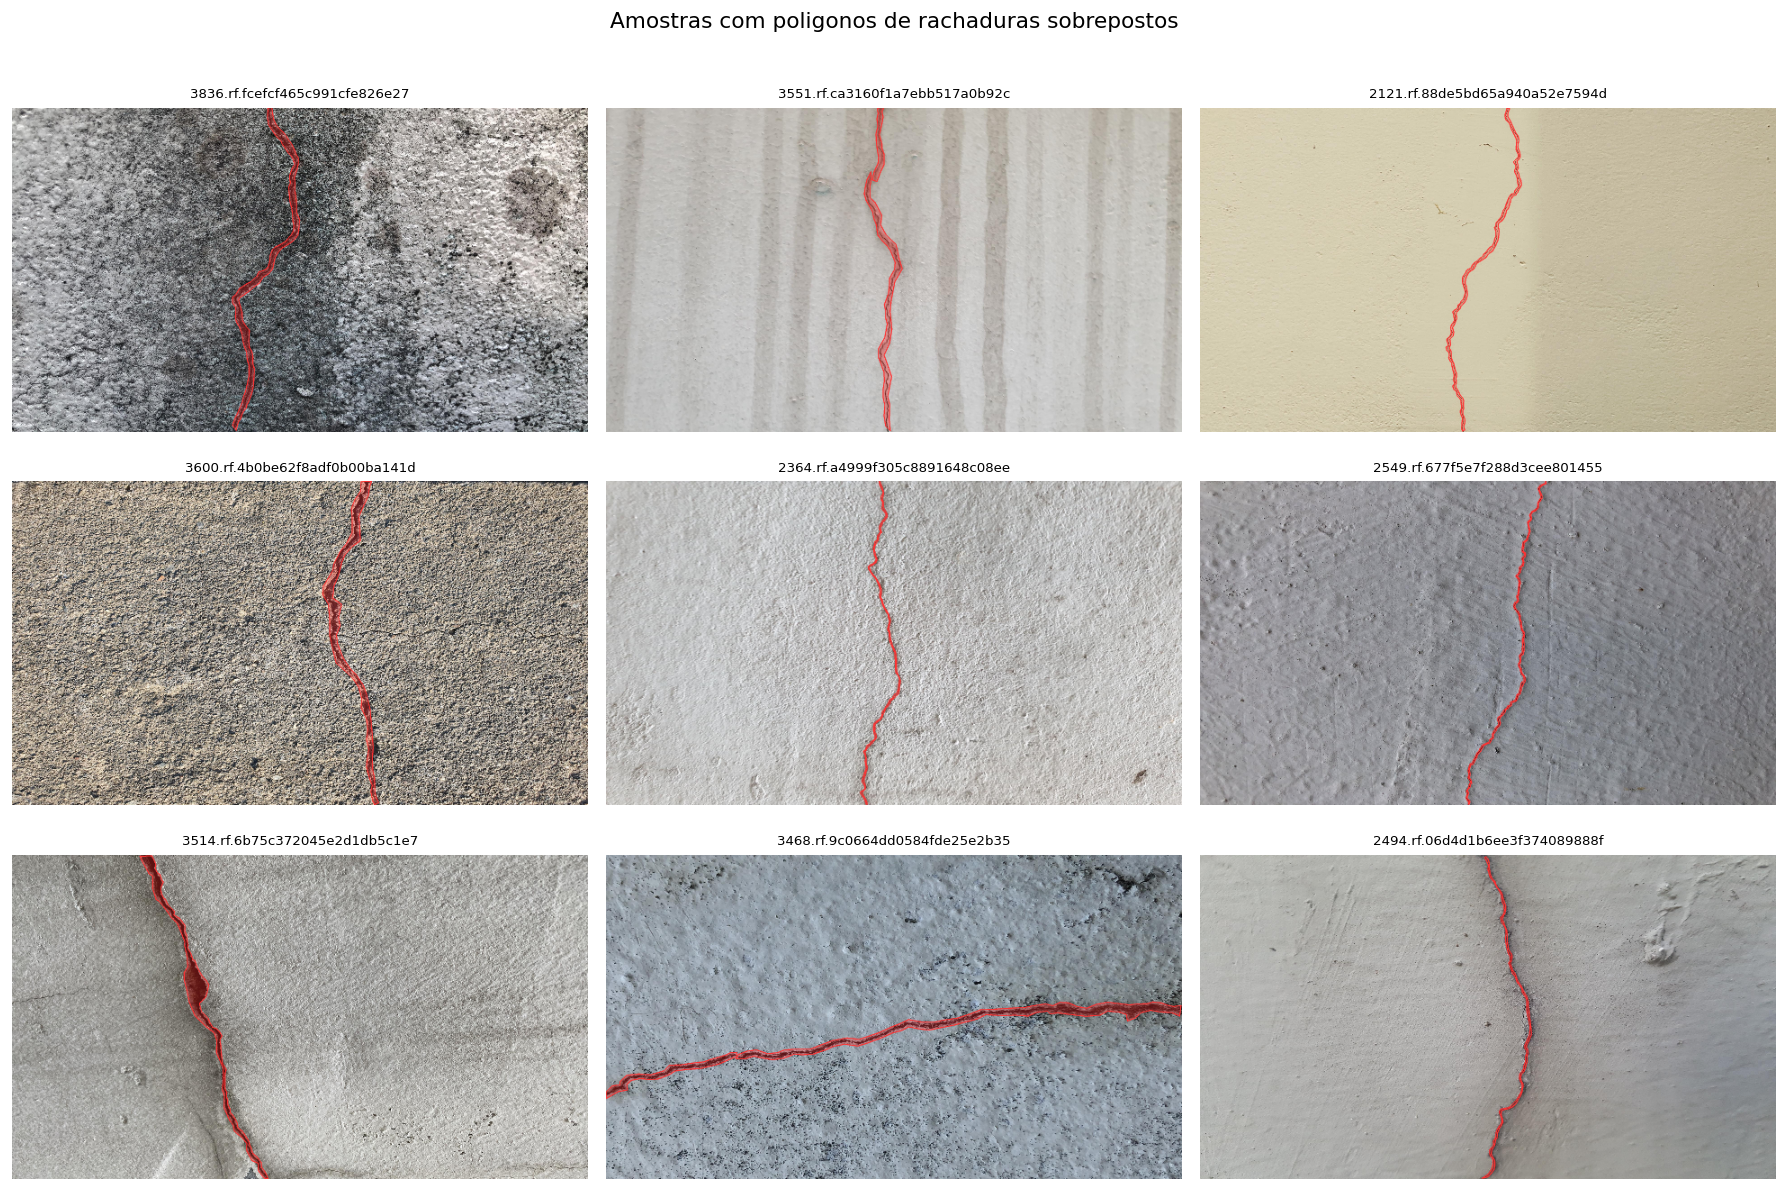
\includegraphics[width=\linewidth]{eda_samples.png}\caption{Amostras anotadas do dataset}
  \end{subfigure}\hfill
  \begin{subfigure}{0.48\linewidth}\centering
    
\includegraphics[width=\linewidth]{eda_distributions.png}\caption{Distribuições das anotações}
  \end{subfigure}
  \\[6pt]
  \begin{subfigure}{0.48\linewidth}\centering
    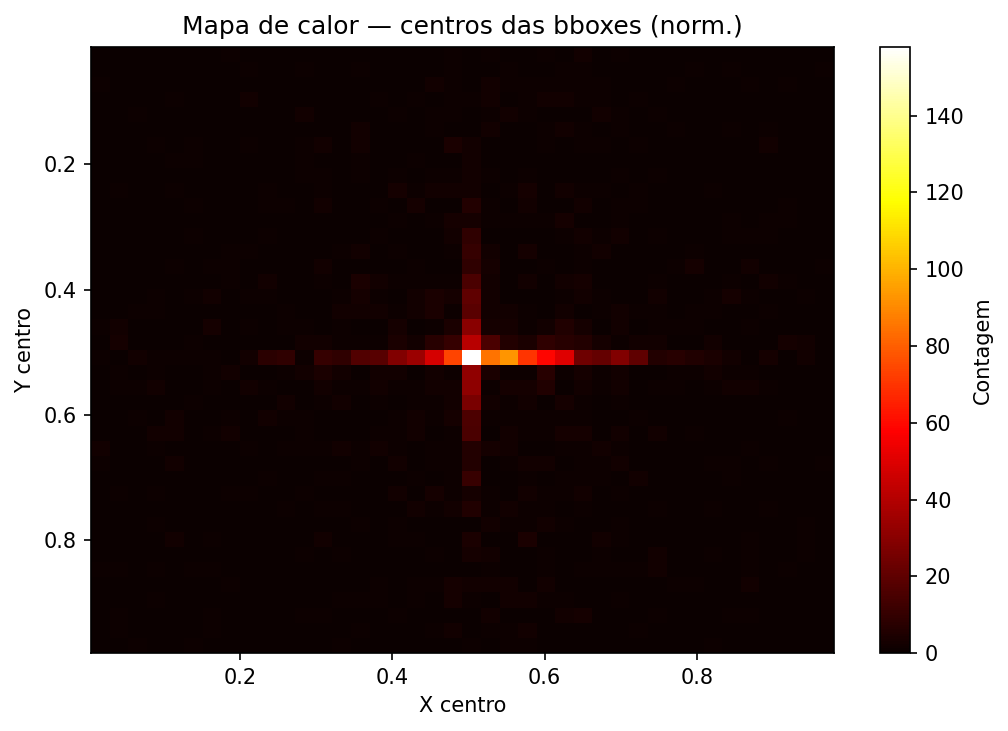
\includegraphics[width=\linewidth]{eda_heatmap.png}\caption{Mapa de calor de posições}
  \end{subfigure}\hfill
  \begin{subfigure}{0.48\linewidth}\centering
    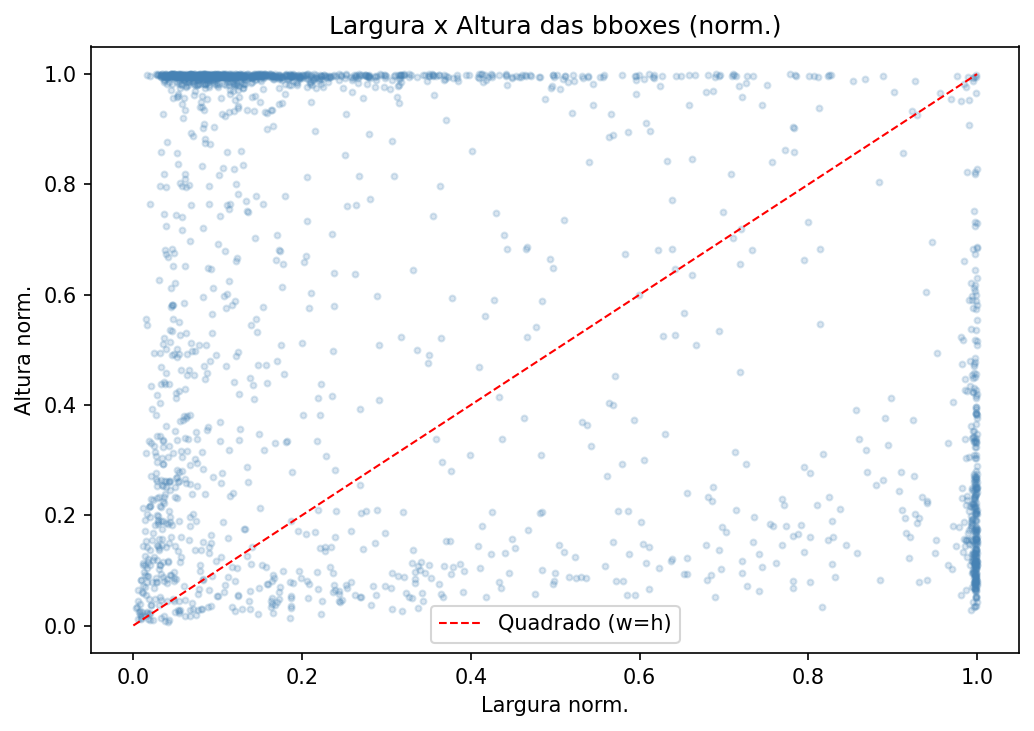
\includegraphics[width=\linewidth]{eda_bbox_scatter.png}\caption{Dispersão largura\,$\times$\,altura}
  \end{subfigure}
  \caption{Análise exploratória do dataset de rachaduras.}
\end{figure}

% ============================================================================
\section{Planejamento — UX/UI e implementação}
% ============================================================================
A solução não é só o modelo: ela precisa ser \textbf{usável por um colaborador em obra}.
Por isso houve um \textbf{processo de planejamento de UX/UI} antes da implementação,
documentado em detalhe no \textbf{guia em PDF à parte}.

\subsection{Processo de planejamento de UX/UI}
O fluxo foi desenhado em torno de um operário/inspetor que precisa, com poucos toques:
\textbf{(1)} se identificar; \textbf{(2)} enviar/capturar a foto da parede; \textbf{(3)} ver o
resultado da IA; \textbf{(4)} registrar no diário de obra; \textbf{(5)} acompanhar indicadores.
Princípios adotados: layout \emph{mobile-first}, navegação inferior fixa, leitura rápida do
status (concluída/alerta) e linguagem do domínio (\emph{rachadura}, \emph{diário de obra},
\emph{inspeção}).

As telas de planejamento (\emph{wireframes}/protótipos de alta fidelidade) que guiaram o
desenvolvimento são apresentadas abaixo.

\begin{figure}[H]\centering
  \begin{subfigure}{0.48\linewidth}\centering
    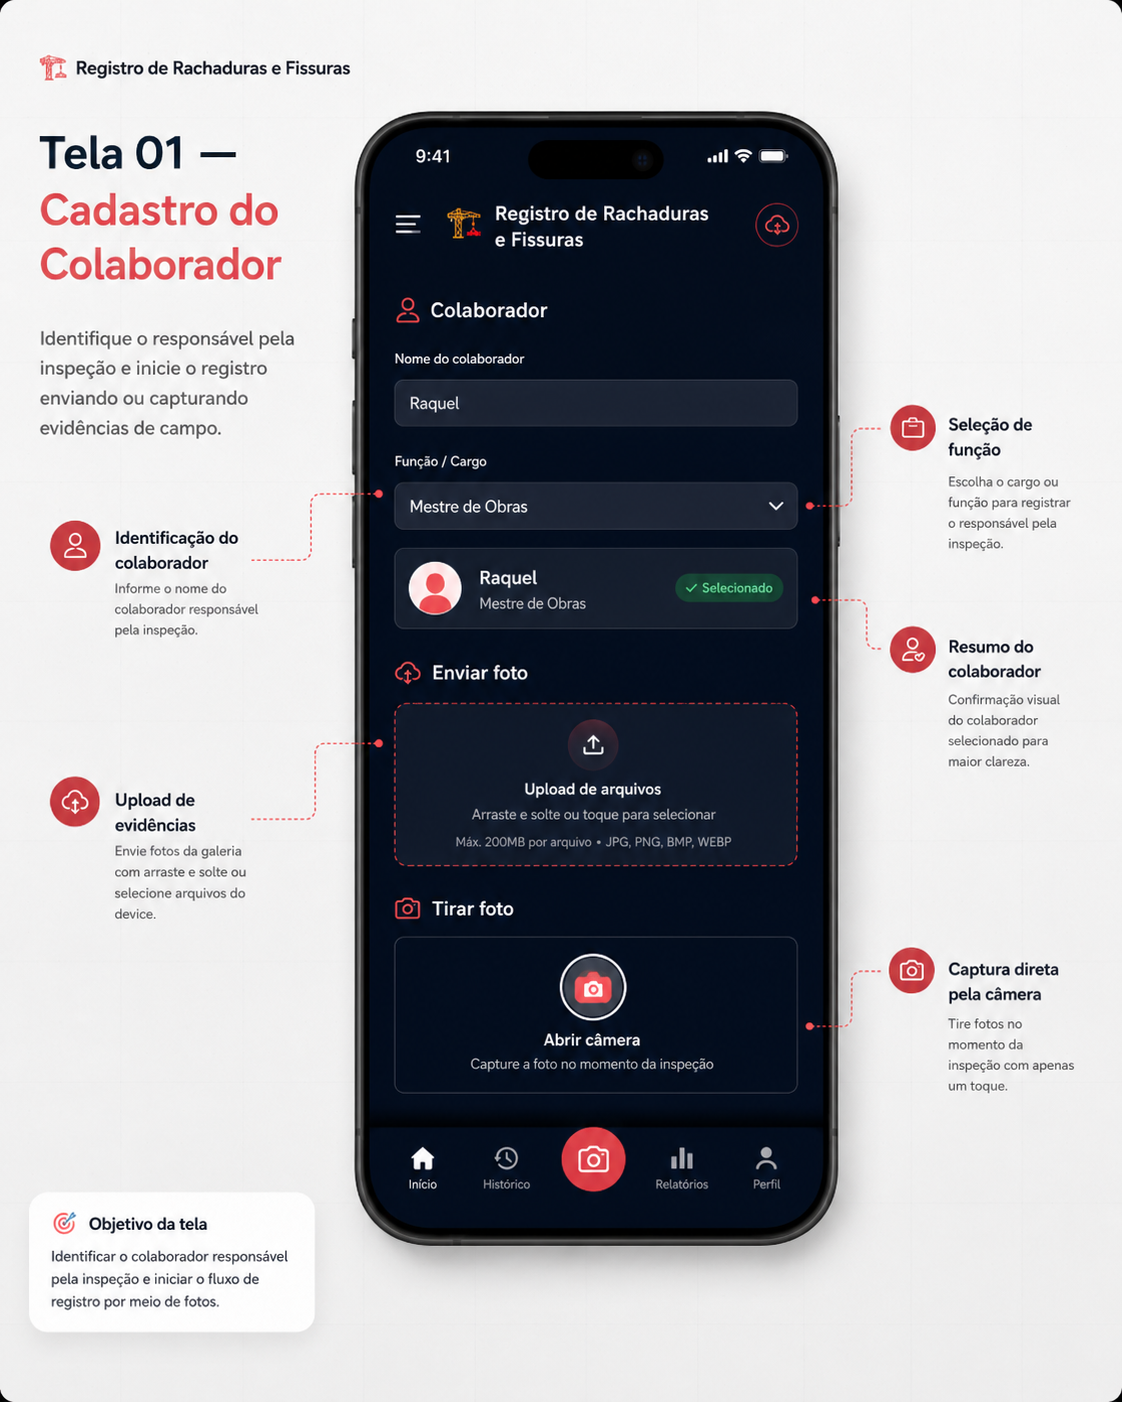
\includegraphics[width=\linewidth]{tela1.png}\caption{Tela 1 — identificação / início}
  \end{subfigure}\hfill
  \begin{subfigure}{0.48\linewidth}\centering
    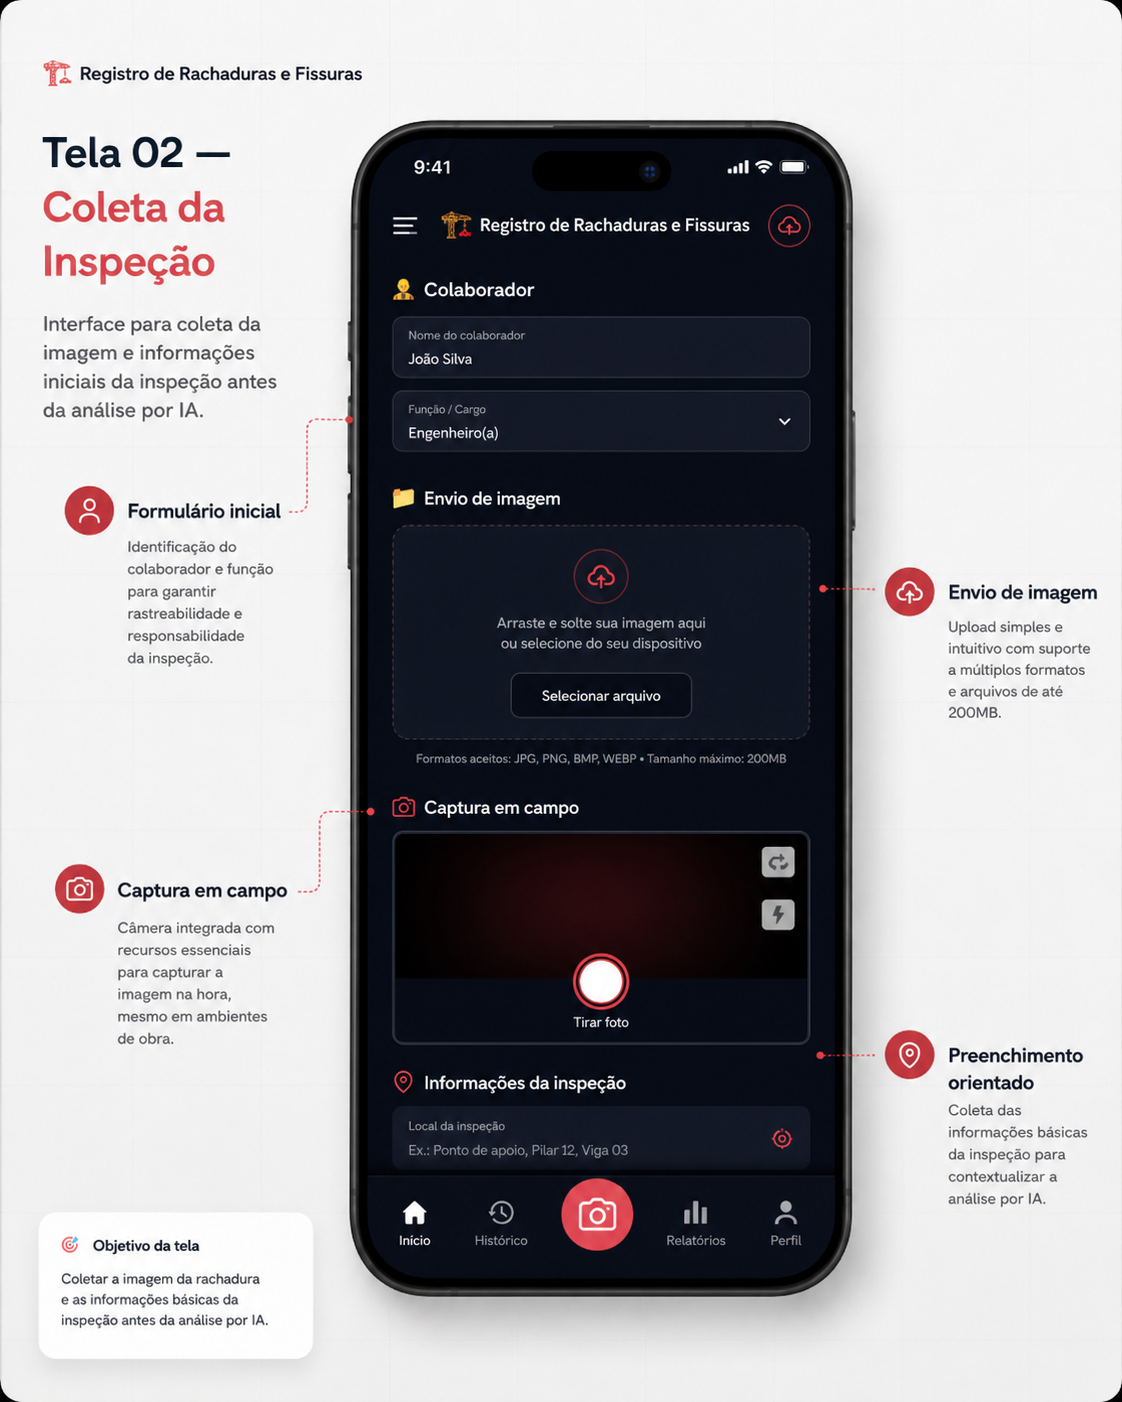
\includegraphics[width=\linewidth]{tela2.png}\caption{Tela 2 — envio / captura da imagem}
  \end{subfigure}
  \\[6pt]
  \begin{subfigure}{0.48\linewidth}\centering
    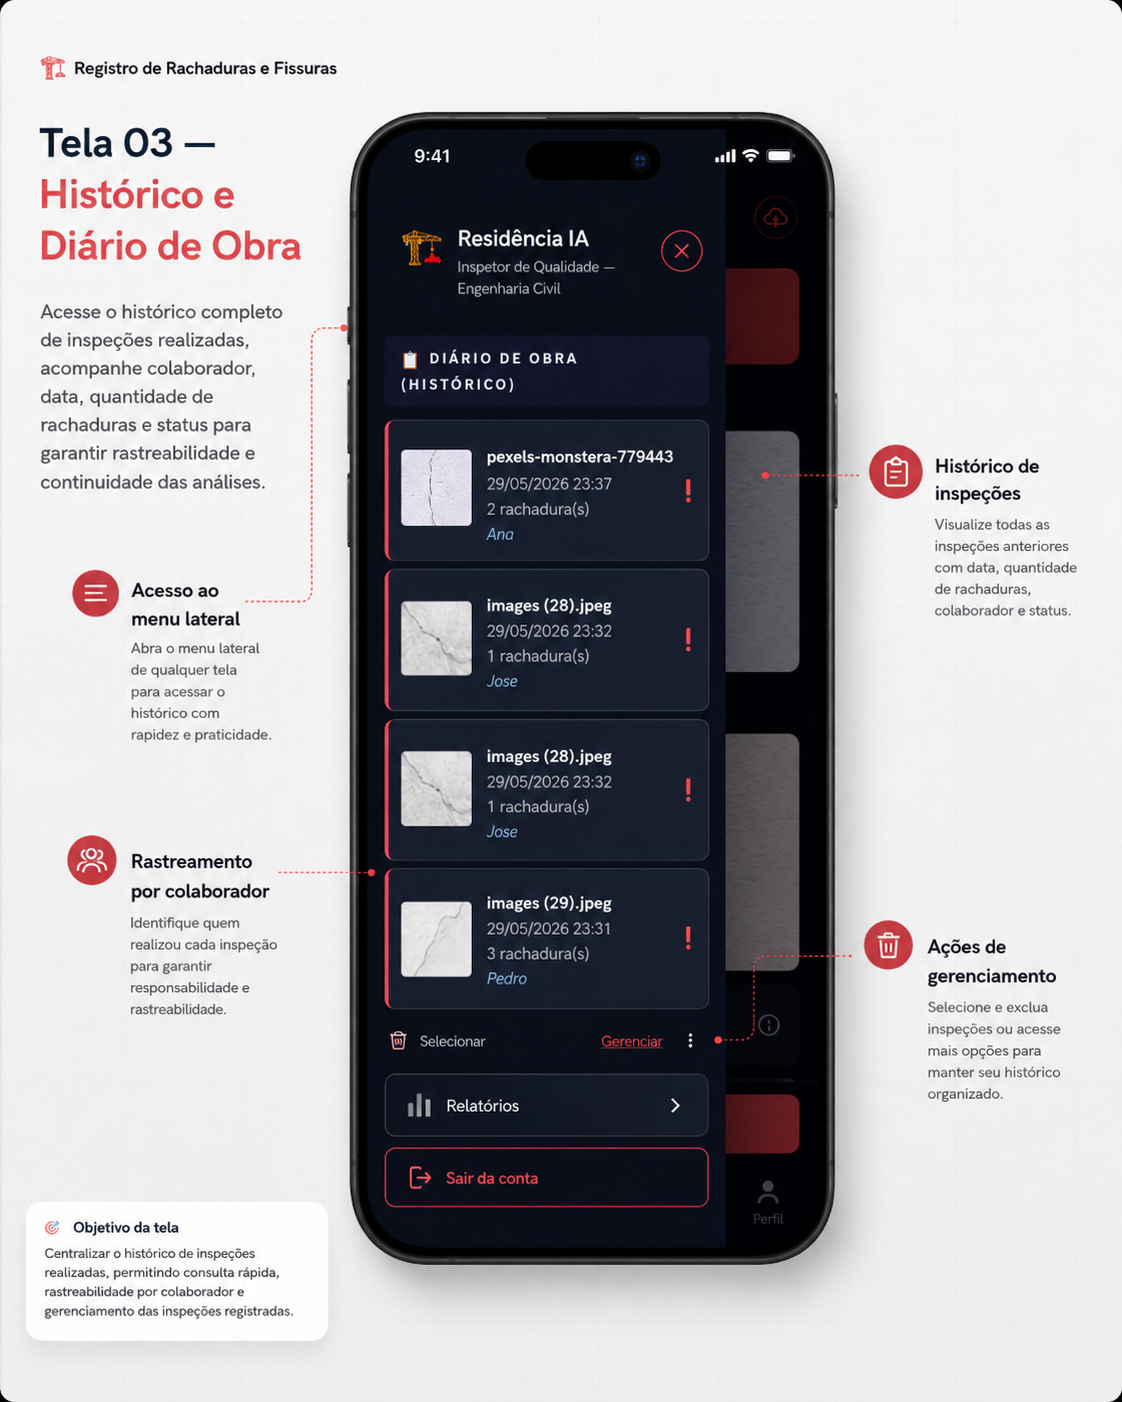
\includegraphics[width=\linewidth]{tela3.png}\caption{Tela 3 — resultado da inspeção}
  \end{subfigure}\hfill
  \begin{subfigure}{0.48\linewidth}\centering
    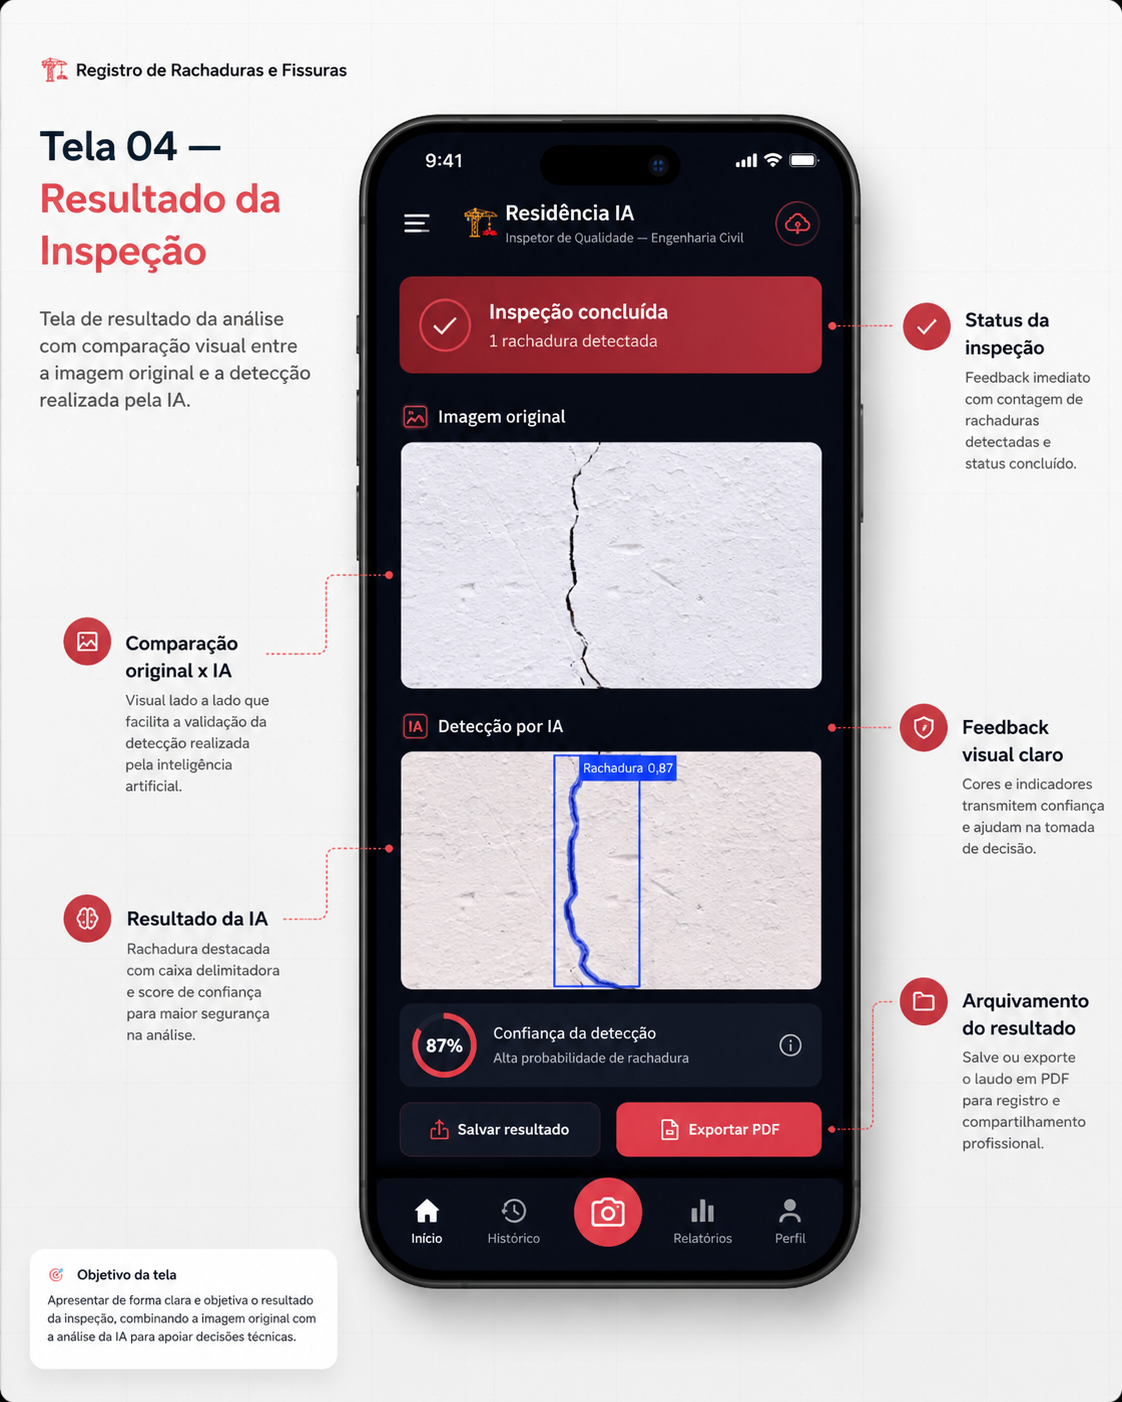
\includegraphics[width=\linewidth]{tela4.png}\caption{Tela 4 — histórico / dashboard}
  \end{subfigure}
  \caption{Planejamento de UX/UI — protótipo das quatro telas principais (tela1 a tela4).}
\end{figure}

\subsection{Como ficou implementado}
A aplicação foi construída em \textbf{Streamlit}, com tema próprio (CSS), navegação inferior e
geração de relatório de inspeção. As capturas reais do app implementado (app-1 a app-5):

\begin{figure}[H]\centering
  \begin{subfigure}{0.32\linewidth}\centering
    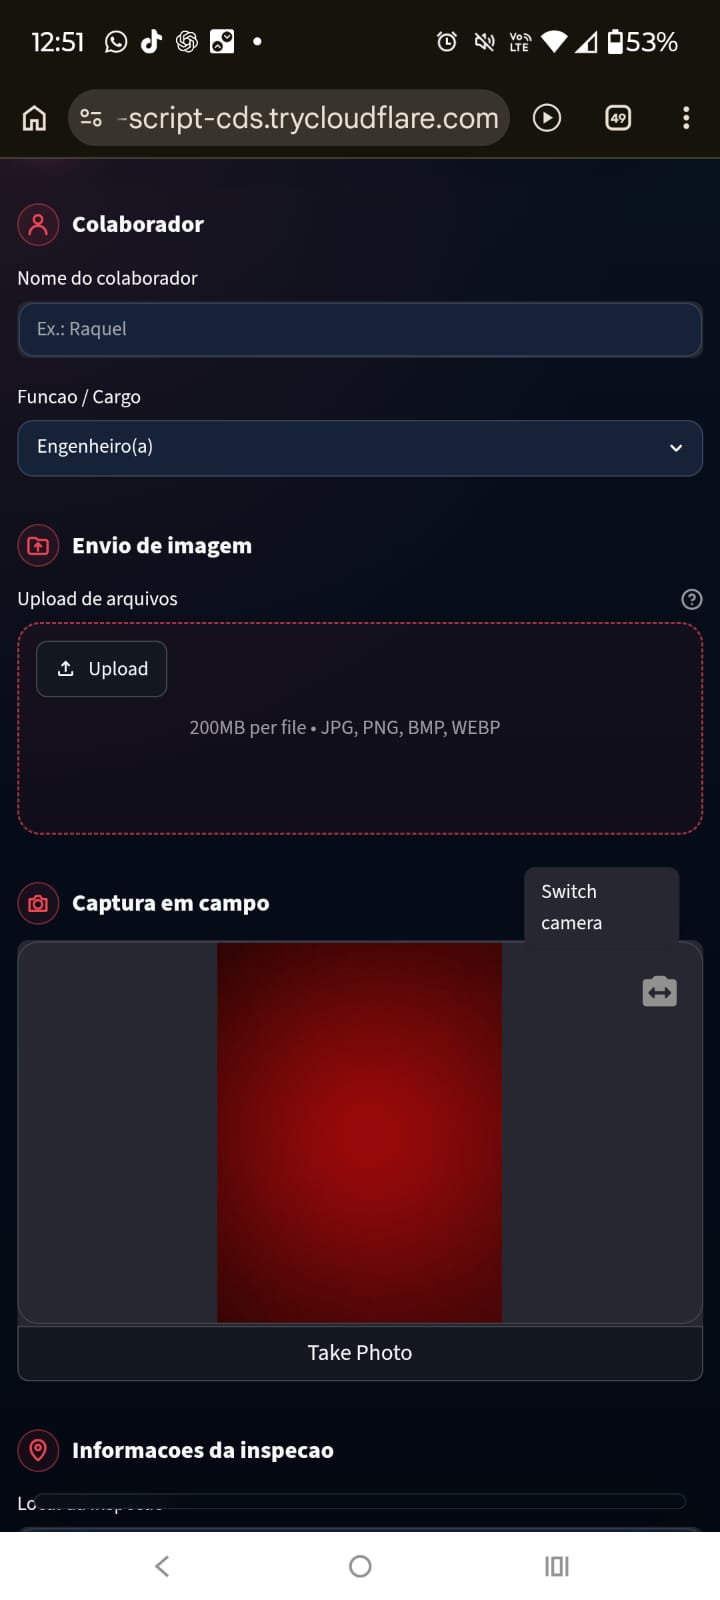
\includegraphics[width=\linewidth]{app-1.jpeg}\caption{app-1 — início/colaborador}
  \end{subfigure}\hfill
  \begin{subfigure}{0.32\linewidth}\centering
    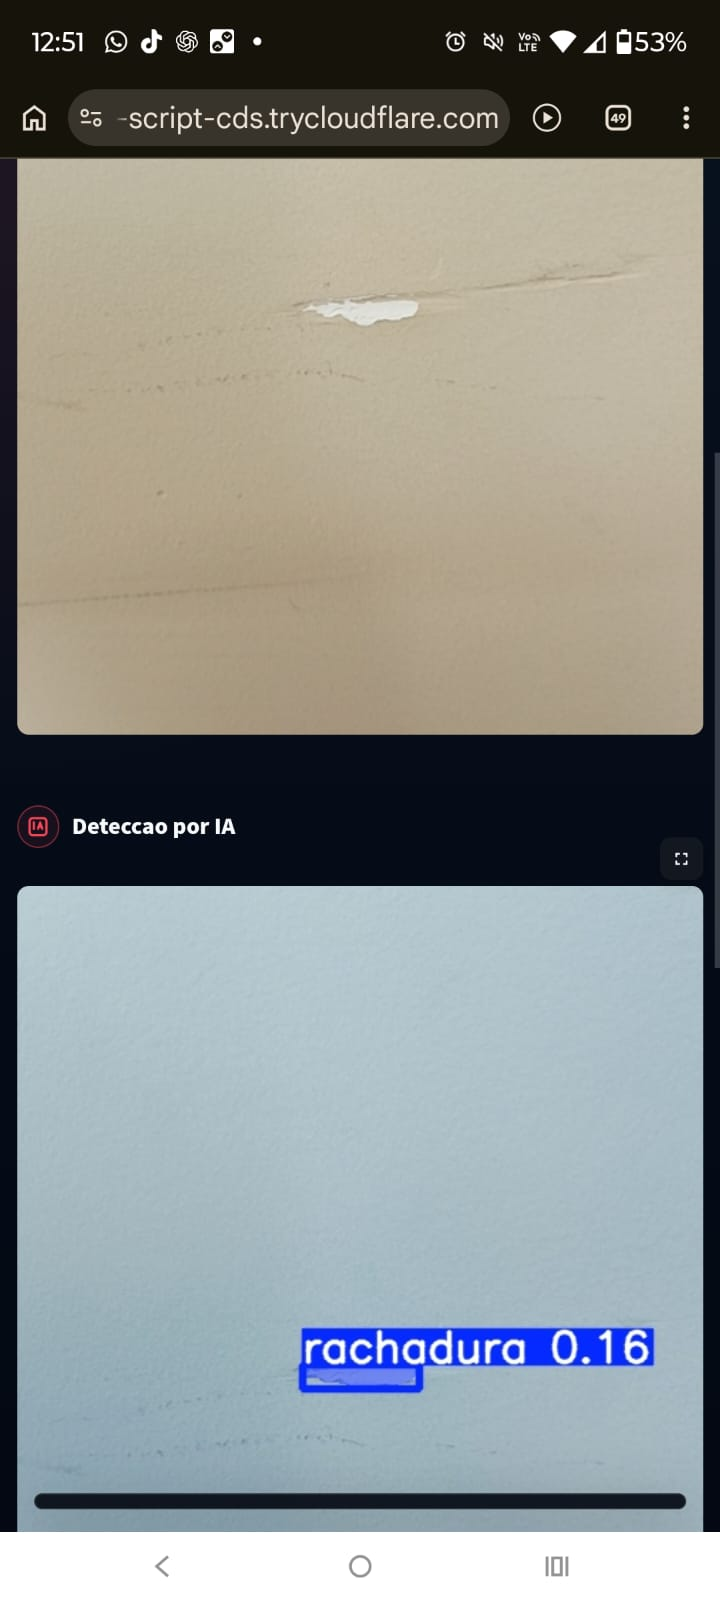
\includegraphics[width=\linewidth]{app-2.jpeg}\caption{app-2 — envio da imagem}
  \end{subfigure}\hfill
  \begin{subfigure}{0.32\linewidth}\centering
    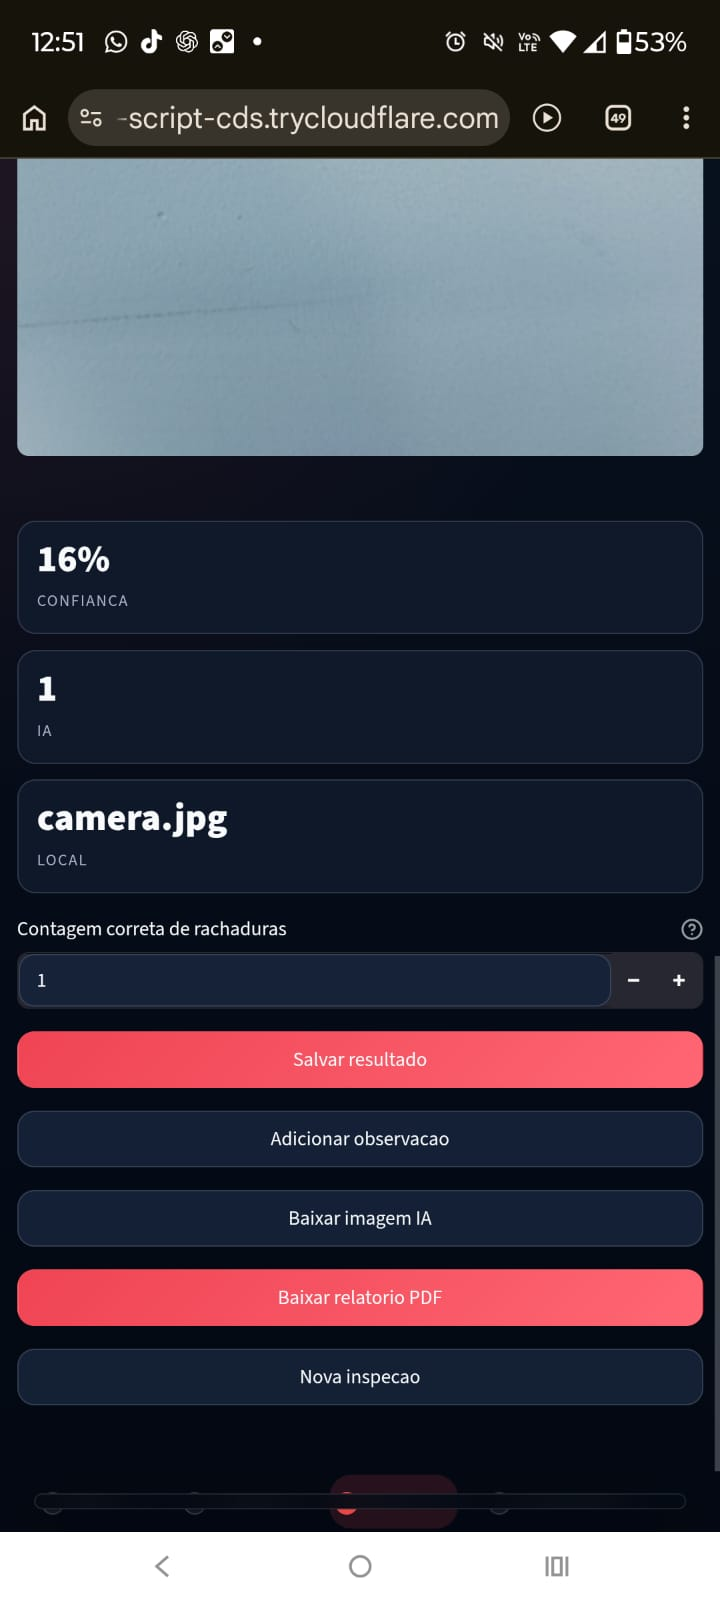
\includegraphics[width=\linewidth]{app-3.jpeg}\caption{app-3 — resultado da IA}
  \end{subfigure}
  \\[6pt]
  \begin{subfigure}{0.32\linewidth}\centering
    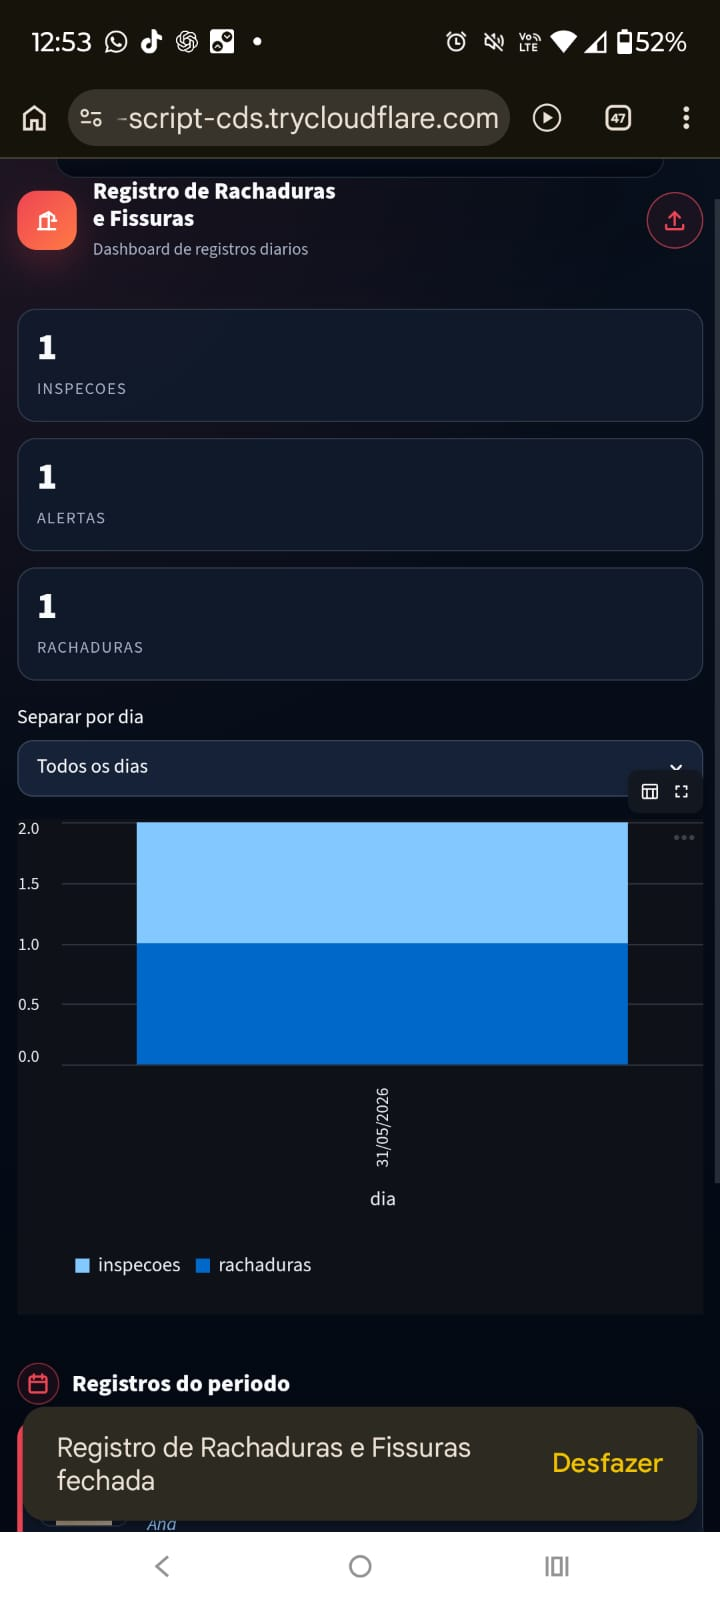
\includegraphics[width=\linewidth]{app-4.jpeg}\caption{app-4 — histórico/diário}
  \end{subfigure}\hfill
  \begin{subfigure}{0.32\linewidth}\centering
    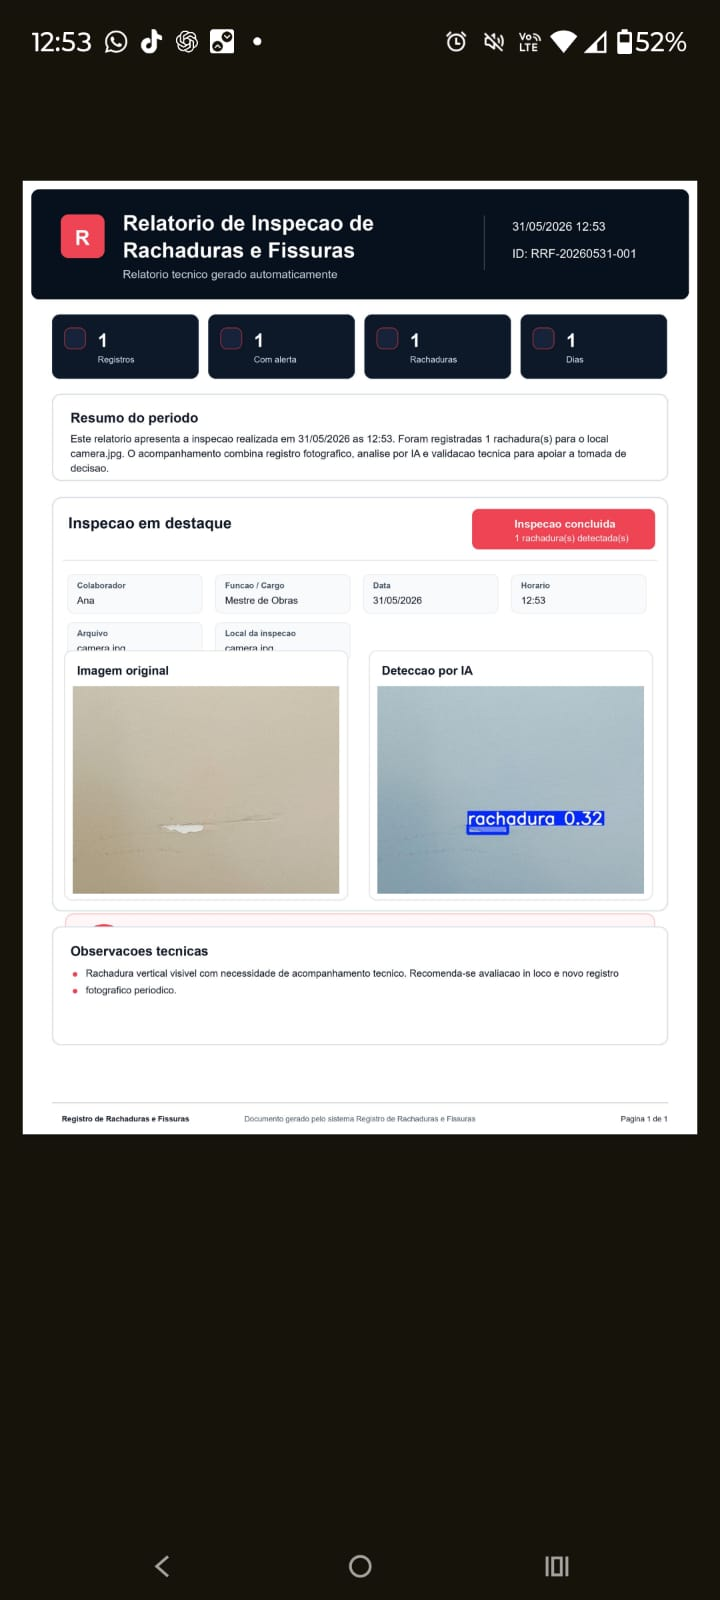
\includegraphics[width=\linewidth]{app-5.jpeg}\caption{app-5 — dashboard}
  \end{subfigure}
  \caption{Implementação final do aplicativo \emph{Inspetor de Qualidade} (app-1 a app-5).}
\end{figure}

\begin{infobox}
\textbf{Funcionalidades do app:} perfil do colaborador (nome/cargo), upload ou câmera,
inferência YOLO com máscara sobreposta, contagem de detecções e confiança, salvamento no
\textbf{histórico/diário de obra}, exportação CSV, \textbf{dashboard} por dia e geração de
\textbf{relatório de inspeção} em imagem/PDF.
\end{infobox}

% ============================================================================
\section{Organização do projeto}
% ============================================================================
O repositório segue um pipeline em etapas, do dado ao deploy:

\begin{table}[H]\centering\small
\renewcommand{\arraystretch}{1.25}
\begin{tabular}{>{\ttfamily}l >{\raggedright\arraybackslash}p{10.5cm}}
\toprule
\textnormal{\textbf{Caminho}} & \textbf{Função} \\
\midrule
src/prepare\_dataset.py & Etapa 1 — split train/val/test (70/20/10) e geração do \texttt{data.yaml} \\
src/train.py            & Etapa 2 — treinamento (augmentations específicas para fissuras) \\
src/evaluate.py         & Etapa 3 — métricas no conjunto de teste (mAP, P, R) \\
src/predict.py          & Etapa 3 — inferência com visualização de máscaras \\
src/export.py           & Etapa 4 — exportação ONNX / TFLite (deploy \emph{edge}) \\
app/app.py              & Etapa 5 — interface Streamlit (Inspetor de Qualidade) \\
models/                 & Pesos treinados (\texttt{.pt}, \texttt{.onnx}, \texttt{.tflite}) \\
results/ — runs/        & Curvas, matrizes de confusão, métricas e inferências \\
\bottomrule
\end{tabular}
\caption{Estrutura do projeto \texttt{desafio2\_trincas/}.}
\end{table}

\begin{table}[H]\centering\small
\renewcommand{\arraystretch}{1.25}
\begin{tabular}{lccc}
\toprule
\textbf{Split} & \textbf{Train} & \textbf{Val} & \textbf{Test} \\
\midrule
Imagens & 1.085 & 310 & 156 \\
Proporção & 70\% & 20\% & 10\% \\
\bottomrule
\end{tabular}
\caption{Particionamento do dataset (1.551 imagens, classe única \texttt{rachadura}).}
\end{table}

% ============================================================================
\section{Métricas do modelo e justificativa da escolha}
% ============================================================================
\subsection{Critérios de decisão}
A avaliação foi feita com critérios explícitos, conforme exige o desafio:
\begin{itemize}[leftmargin=1.4em]
  \item \textbf{Confiança \(\geq 0{,}25\)}: uma detecção só é aceita se a confiança for de pelo
        menos 25\% (padrão YOLO na avaliação).
  \item \textbf{IoU \(\geq 0{,}50\)}: um verdadeiro positivo exige sobreposição de pelo menos
        50\% entre predição e \emph{ground truth} — é exatamente o \textbf{mAP@0.5}.
  \item No \textbf{aplicativo em produção}, a confiança é reduzida para \(0{,}15\) e IoU \(0{,}45\):
        em campo, prioriza-se \textbf{não perder fissuras} (recall) mesmo ao custo de algum falso
        positivo, que o inspetor descarta visualmente.
\end{itemize}

\subsection{Por que essas métricas}
\begin{table}[H]\centering\small
\renewcommand{\arraystretch}{1.3}
\begin{tabular}{>{\bfseries}l >{\raggedright\arraybackslash}p{10.8cm}}
\toprule
Métrica & Por que é adequada ao problema \\
\midrule
Precision & Quanto das detecções são reais. Importa porque texturas/sombras geram falsos
positivos; baixa precision gera retrabalho do inspetor. \\
Recall & Quanto das trincas reais foram encontradas. \textbf{Crítica} em segurança: uma fissura
não detectada é um risco que passa despercebido. \\
mAP@0.5 & Métrica padrão de detecção; resume P\,$\times$\,R ao longo dos limiares com IoU\,$\geq$\,0,5.
Boa leitura geral de qualidade de localização. \\
mAP@0.5:0.95 & Mais rigorosa (média sobre vários IoU). Para máscara fica baixa por natureza:
exigir alta sobreposição em objetos com poucos pixels (fissuras finas) é severo. \\
F1 (Box/Mask) & Equilíbrio P\,$\times$\,R; usada para escolher o limiar de confiança operacional. \\
Matriz de confusão & Mostra o balanço entre acertos e o fundo (\emph{background}) — onde estão
os falsos positivos/negativos. \\
\bottomrule
\end{tabular}
\caption{Justificativa das métricas escolhidas.}
\end{table}

\subsection{Resultados validados no conjunto de teste}
Valores extraídos de \texttt{metrics\_summary.json} (split \texttt{test}, 156 imagens,
conf=0,25, IoU=0,50). \textbf{Métricas conferidas e corretas.}

\begin{table}[H]\centering\small
\renewcommand{\arraystretch}{1.35}
\begin{tabular}{l cc cc}
\toprule
& \multicolumn{2}{c}{\textbf{V1 — 640px}} & \multicolumn{2}{c}{\textbf{V3 — 1280px (produção)}}\\
\cmidrule(lr){2-3}\cmidrule(lr){4-5}
\textbf{Métrica} & \textbf{Box} & \textbf{Mask} & \textbf{Box} & \textbf{Mask}\\
\midrule
mAP@0.5        & 73,2\% & 60,5\% & \textbf{75,8\%} & 58,6\% \\
mAP@0.5:0.95   & 56,7\% & 19,5\% & \textbf{57,7\%} & 19,2\% \\
Precision      & 86,1\% & 77,8\% & \textbf{86,8\%} & 76,4\% \\
Recall         & 72,4\% & 65,5\% & \textbf{74,4\%} & 64,0\% \\
\bottomrule
\end{tabular}
\caption{Métricas no conjunto de teste. O modelo V3 (1280px) foi escolhido para produção por
melhor desempenho de \emph{caixa} (localização) e maior recall — prioridade em inspeção.}
\end{table}

\begin{infobox}
\textbf{Leitura.} Precision de caixa de \(\sim\)87\% indica poucos alarmes falsos; recall de
\(\sim\)74\% confirma boa cobertura das trincas reais. A \(mAP@0.5{:}0.95\) de máscara baixa
(\(\sim\)19\%) é esperada: exigir sobreposição pixel-a-pixel muito alta em objetos finos é
intrinsecamente difícil e \emph{não} indica falha do modelo para o uso pretendido (localizar e
sinalizar a trinca).
\end{infobox}

\subsection{Métricas de rede neural — matrizes de confusão e curvas}
\begin{figure}[H]\centering
  \begin{subfigure}{0.48\linewidth}\centering
    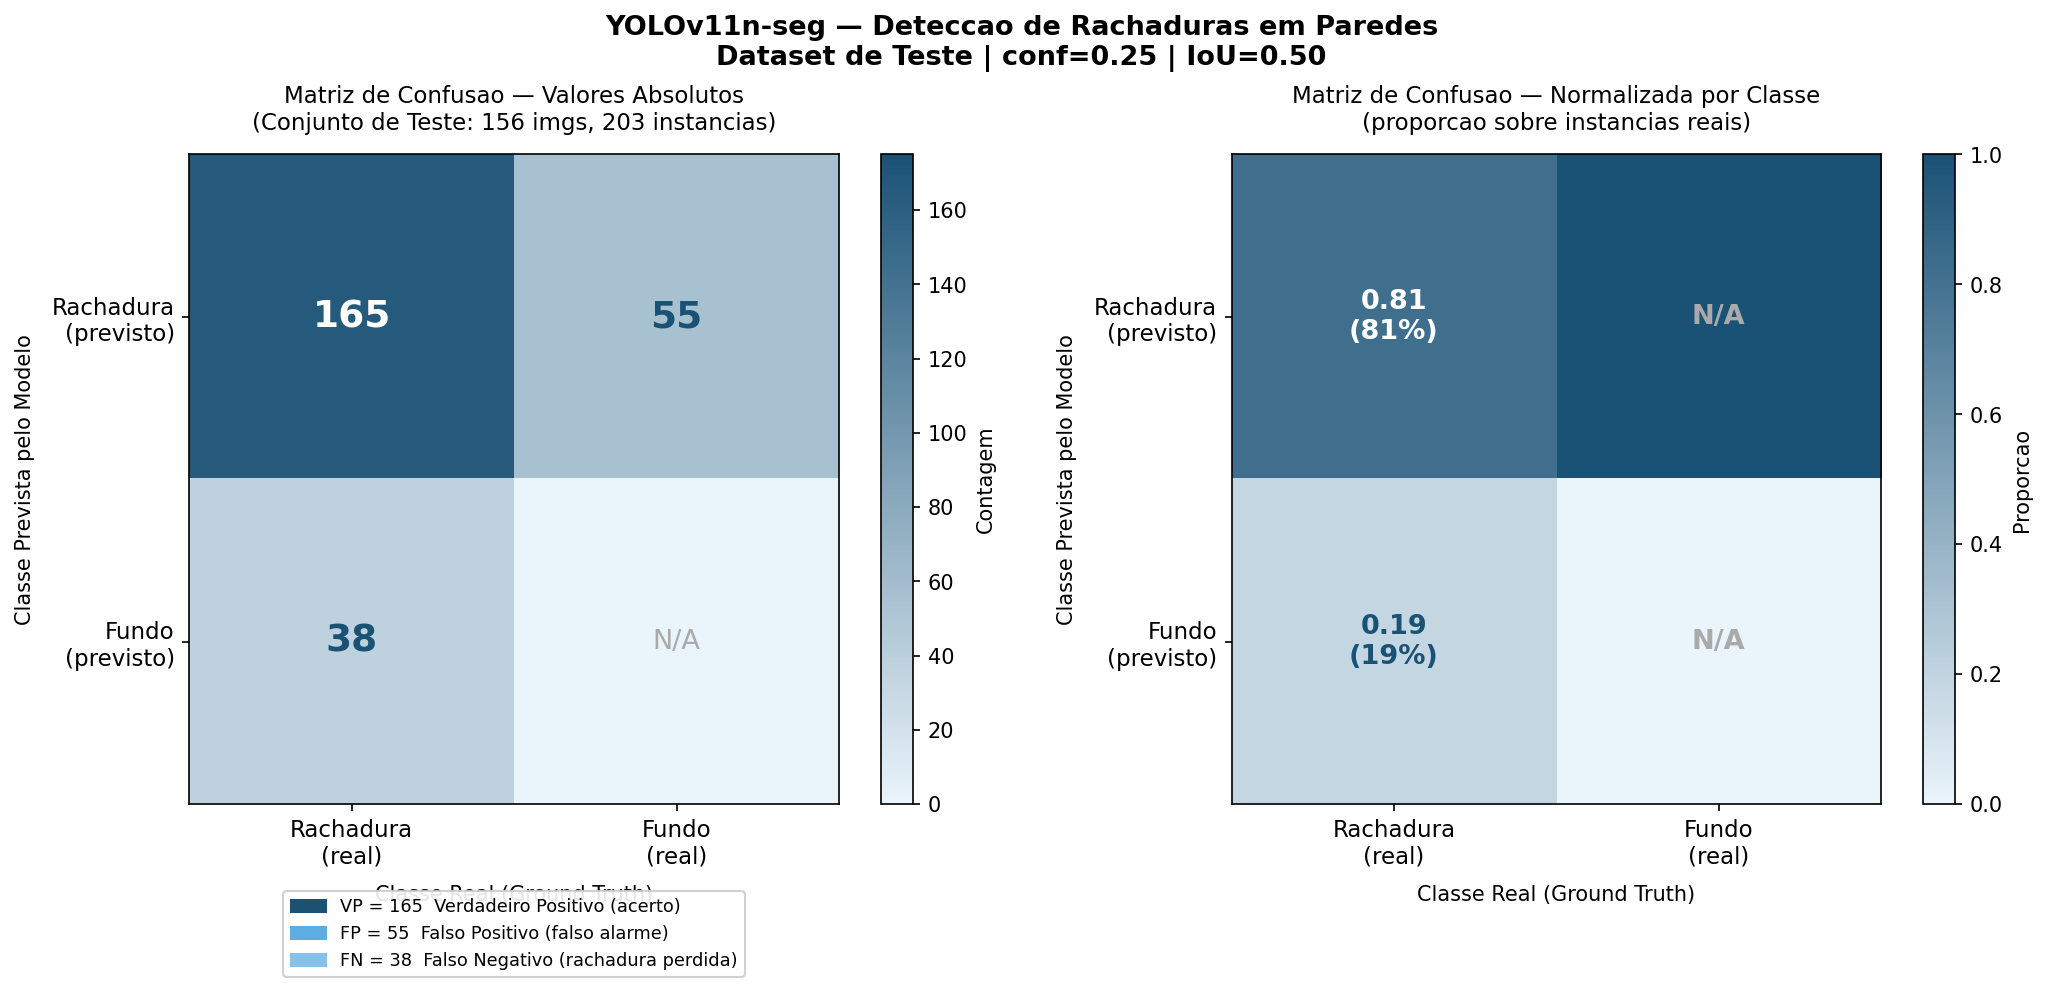
\includegraphics[width=\linewidth]{matriz_confusao_pt.png}\caption{Matriz de confusão (PT)}
  \end{subfigure}\hfill
  \begin{subfigure}{0.48\linewidth}\centering
    
\includegraphics[width=\linewidth]{confusion_matrix_normalized.png}\caption{Matriz normalizada}
  \end{subfigure}
  \caption{Matrizes de confusão — balanço entre rachadura e fundo.}
\end{figure}

\begin{figure}[H]\centering
  \begin{subfigure}{0.48\linewidth}\centering
    
\includegraphics[width=\linewidth]{BoxF1_curve.png}\caption{F1 $\times$ confiança (Box)}
  \end{subfigure}\hfill
  \begin{subfigure}{0.48\linewidth}\centering
    
\includegraphics[width=\linewidth]{BoxPR_curve.png}\caption{Precision $\times$ Recall (Box)}
  \end{subfigure}
  \\[6pt]
  \begin{subfigure}{0.48\linewidth}\centering
    
\includegraphics[width=\linewidth]{BoxP_curve.png}\caption{Precision $\times$ confiança}
  \end{subfigure}\hfill
  \begin{subfigure}{0.48\linewidth}\centering
    
\includegraphics[width=\linewidth]{BoxR_curve.png}\caption{Recall $\times$ confiança}
  \end{subfigure}
  \caption{Curvas de avaliação — usadas para definir o limiar de confiança operacional.}
\end{figure}

% ============================================================================
\section{Resultados gerados pelo modelo}
% ============================================================================
\subsection{Treinamento e convergência}
\fig{results.png}{1.0}{Curvas de treino/validação ao longo das épocas (perdas e métricas).
Convergência estável, sem sinais de \emph{overfitting} severo (early stopping ativo).}

\begin{figure}[H]\centering
  \begin{subfigure}{0.48\linewidth}\centering
    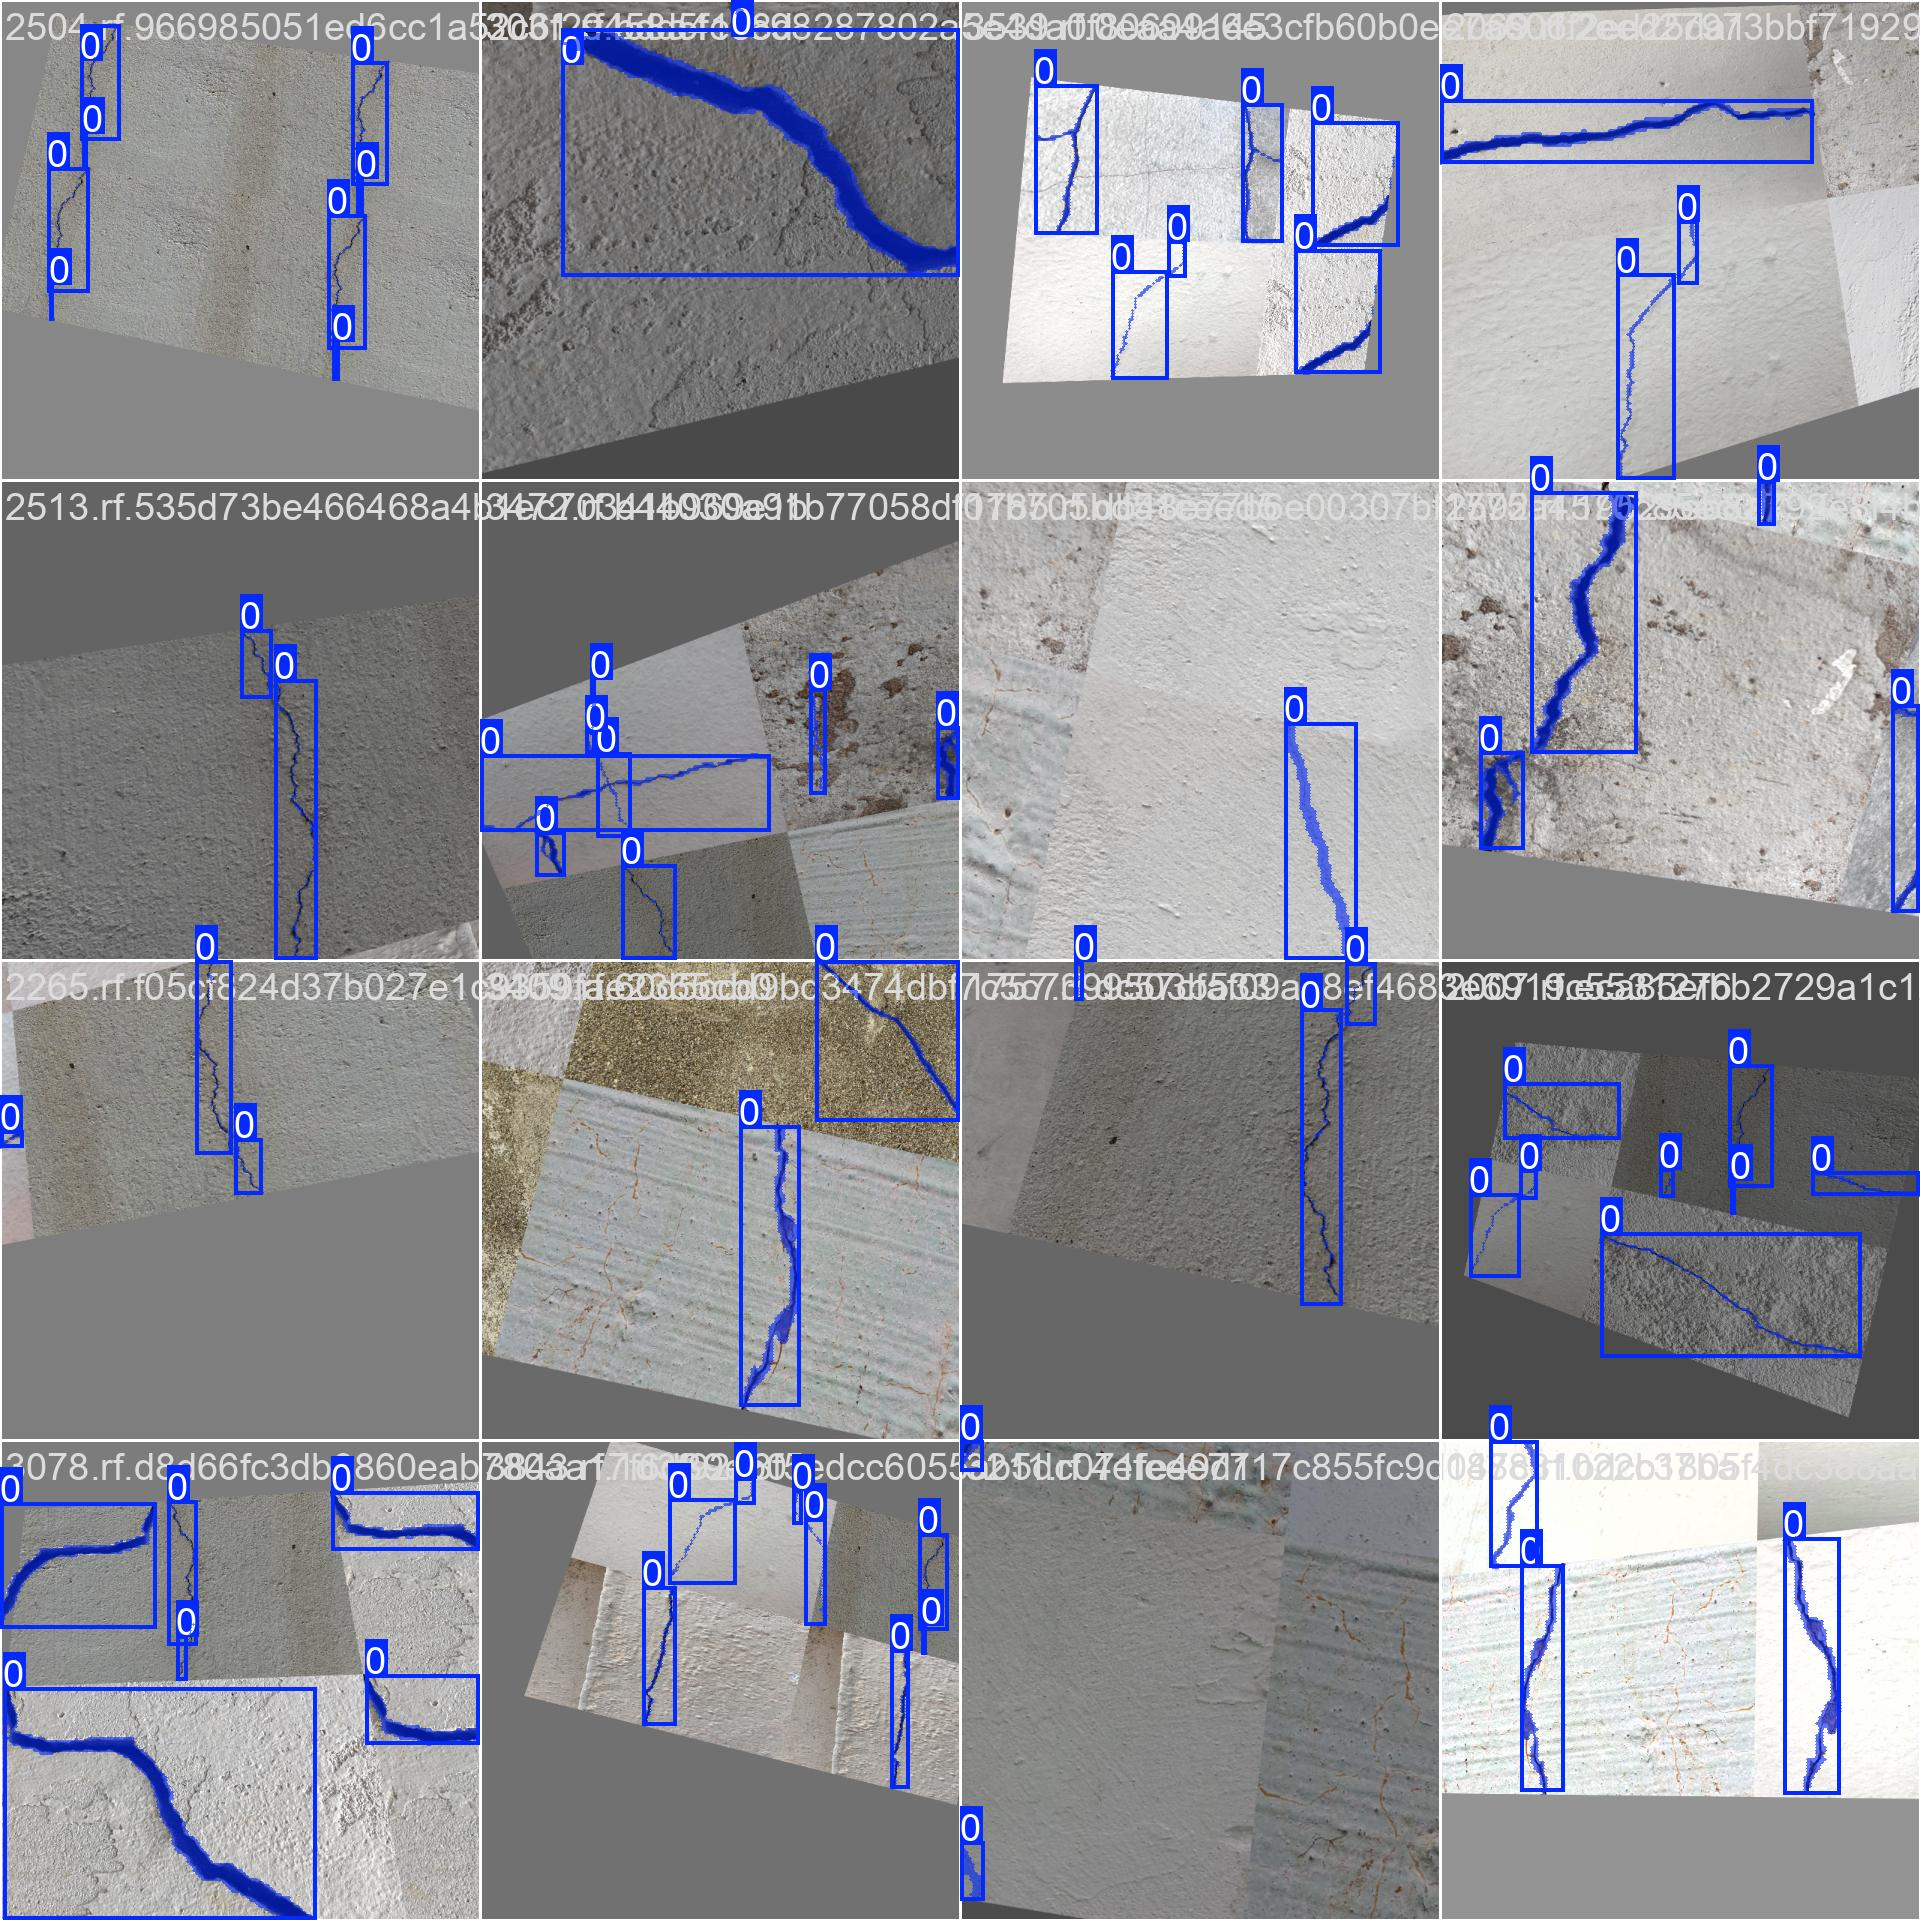
\includegraphics[width=\linewidth]{train_batch0.jpg}\caption{Lote de treino com augmentations}
  \end{subfigure}\hfill
  \begin{subfigure}{0.48\linewidth}\centering
    
\includegraphics[width=\linewidth]{val_batch2_pred.jpg}\caption{Predições em lote de validação}
  \end{subfigure}
  \caption{Exemplos de lotes de treino (augmentations) e de predição em validação.}
\end{figure}

{\sloppy
\paragraph{Configuração de treino (V3, produção).} \texttt{yolo11n-seg.pt}, 150 épocas,
\texttt{imgsz=1280}, \texttt{batch=8}, otimizador \emph{auto}, \texttt{cos\_lr=True}.
Augmentations específicas para fissuras: \texttt{copy\_paste=0.5}, \texttt{degrees=20},
\texttt{fliplr=0.5}, \texttt{flipud=0.3}, \texttt{erasing=0.2} (reduzido para não apagar pixels
de fissuras finas), \texttt{mixup=0.0} (mistura prejudica bordas finas).
\par}

\subsection{Comparação entre modelos (V1 \emph{vs} V3)}
\begin{notebox}
\textbf{Observação.} A imagem \texttt{grid\_resultados\_v3.png} citada não foi localizada na
pasta; foram usadas as imagens de comparação efetivamente disponíveis
(\texttt{comparacao\_v1\_vs\_v3.jpg}, \texttt{comparativo\_v1\_v3.png},
\texttt{comparacao\_modelos\_notebook.png}).
\end{notebox}

\fig{comparativo_v1_v3.png}{0.95}{Comparativo quantitativo V1 (640px) \emph{vs} V3 (1280px).}

\begin{figure}[H]\centering
  \begin{subfigure}{0.49\linewidth}\centering
    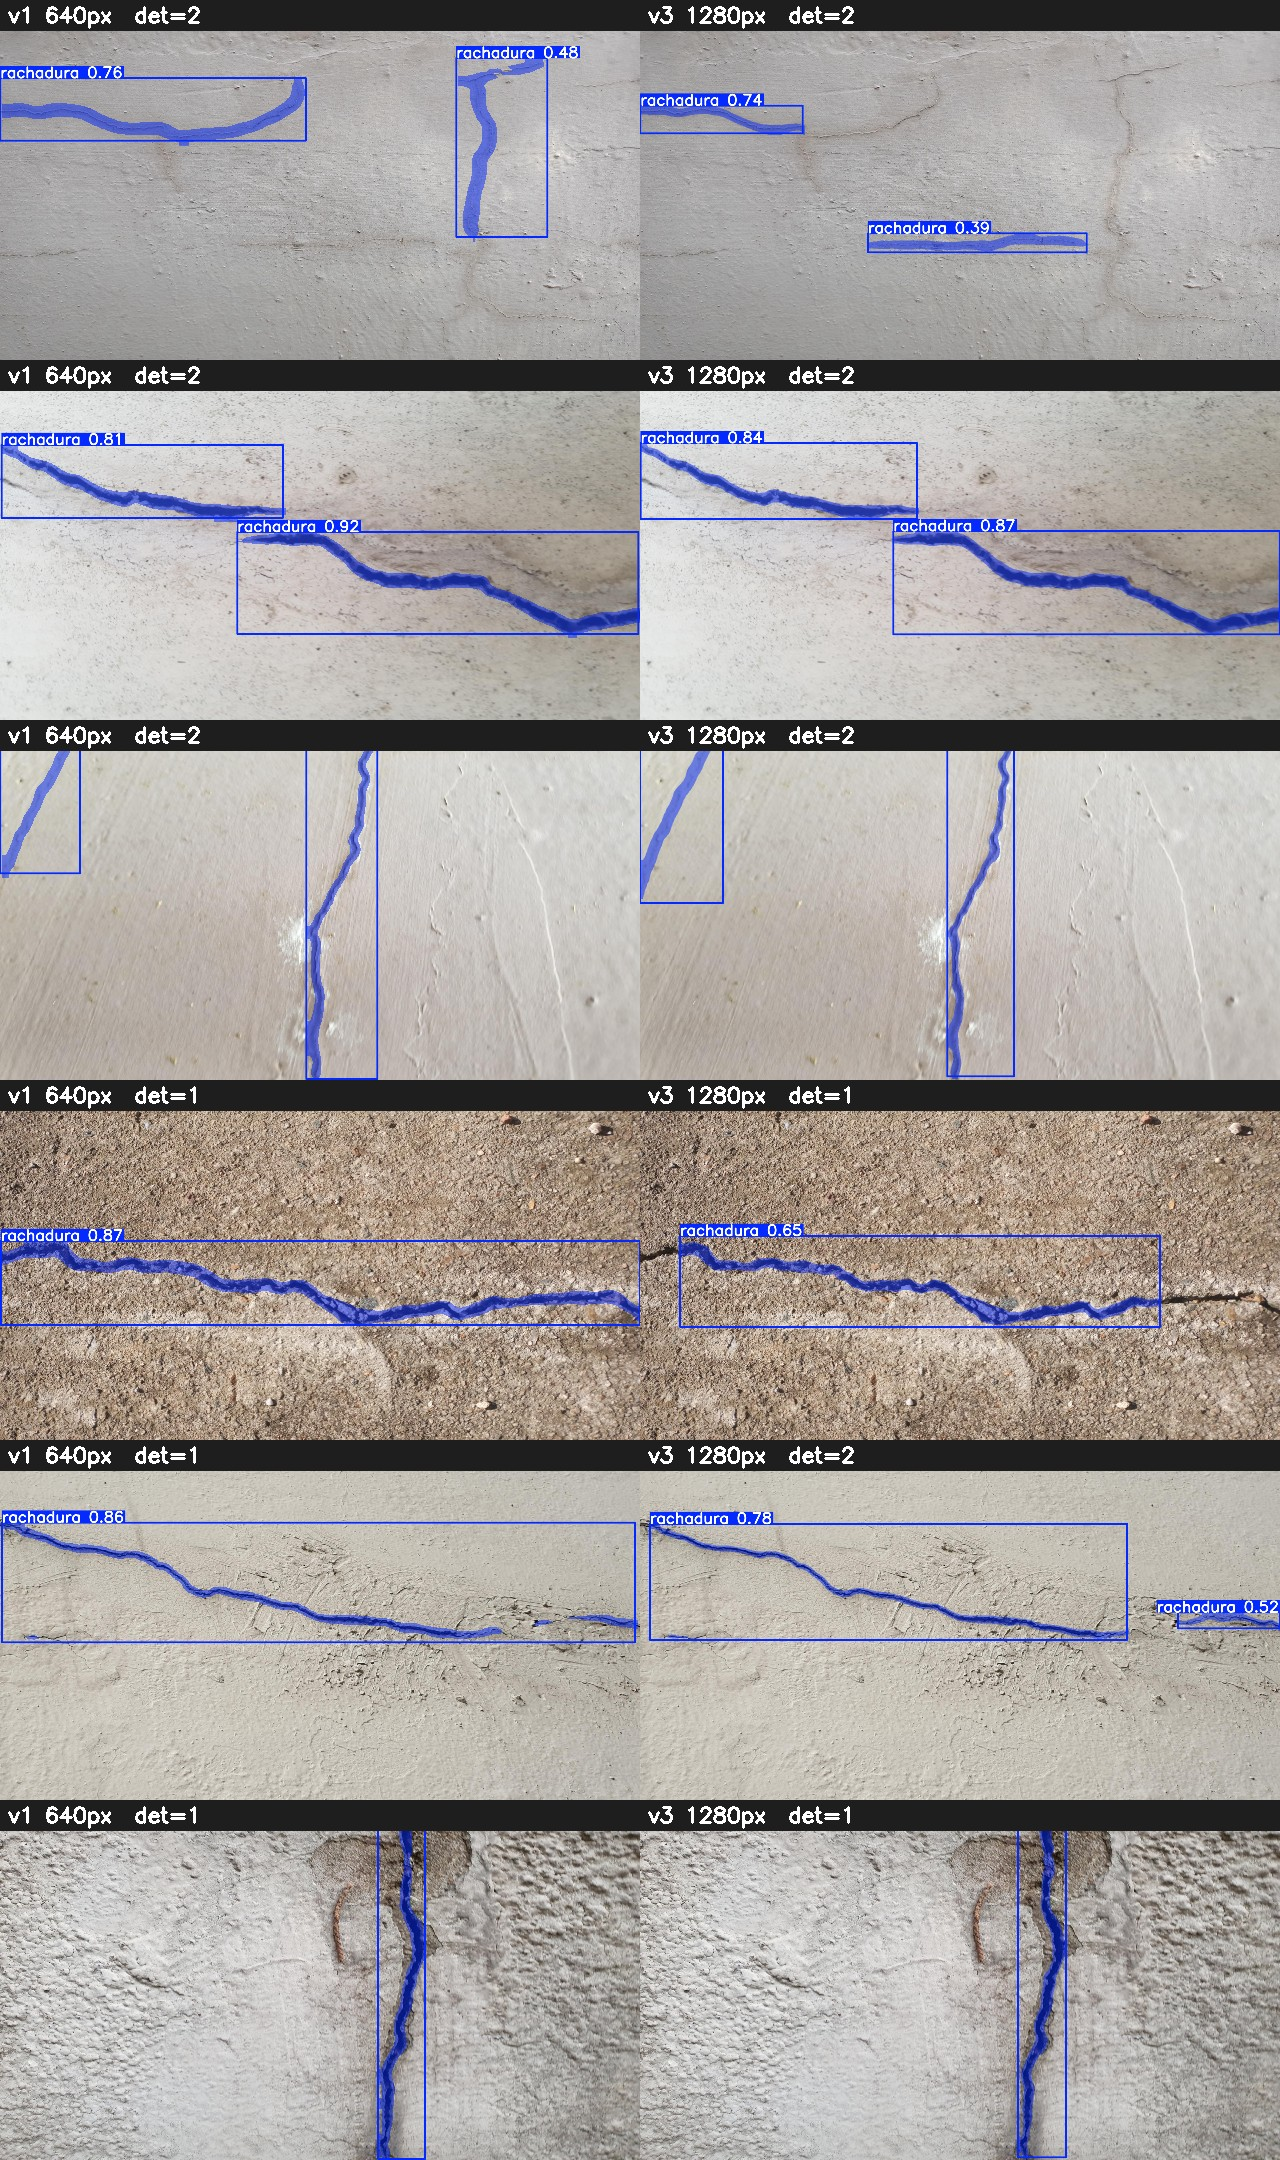
\includegraphics[width=\linewidth]{comparacao_v1_vs_v3.jpg}\caption{Comparação visual V1 \emph{vs} V3}
  \end{subfigure}\hfill
  \begin{subfigure}{0.49\linewidth}\centering
    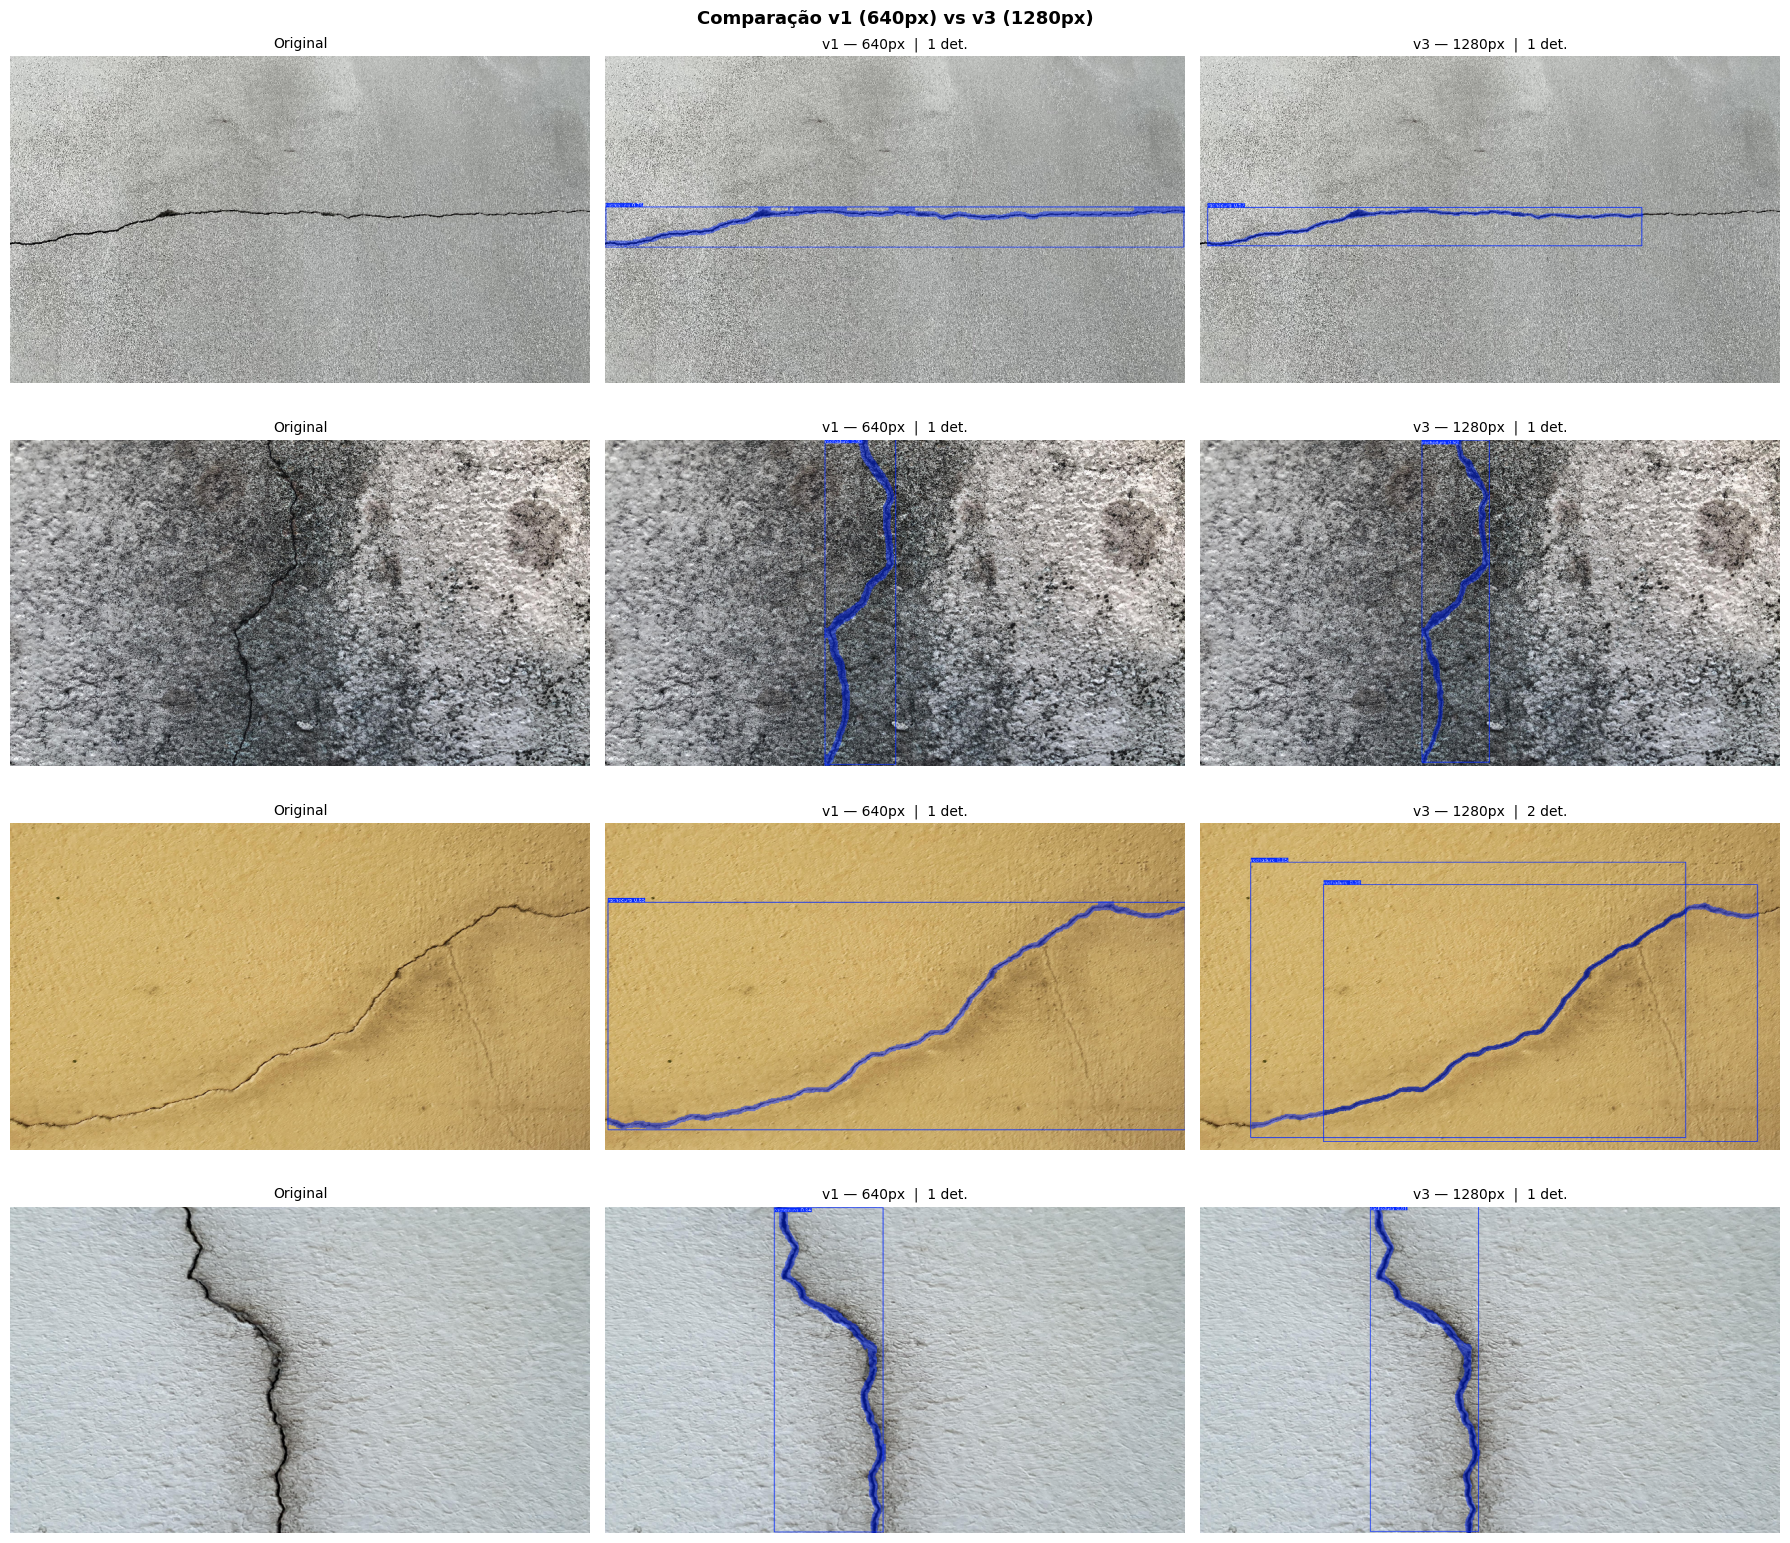
\includegraphics[width=\linewidth]{comparacao_modelos_notebook.png}\caption{Comparação no notebook}
  \end{subfigure}
  \caption{Comparações qualitativas e quantitativas entre as versões do modelo.}
\end{figure}

\fig{inferencia_notebook.png}{0.95}{Inferência no notebook — máscaras de segmentação sobre
imagens de teste.}

% ============================================================================
\section{Aplicação — resultados na prática}
% ============================================================================
Testes em imagens novas (não vistas no treino) demonstram o comportamento do modelo em campo
dentro do aplicativo. Abaixo, resultados de inspeção reais (result-1 a result-3).

\begin{figure}[H]\centering
  \begin{subfigure}{0.32\linewidth}\centering
    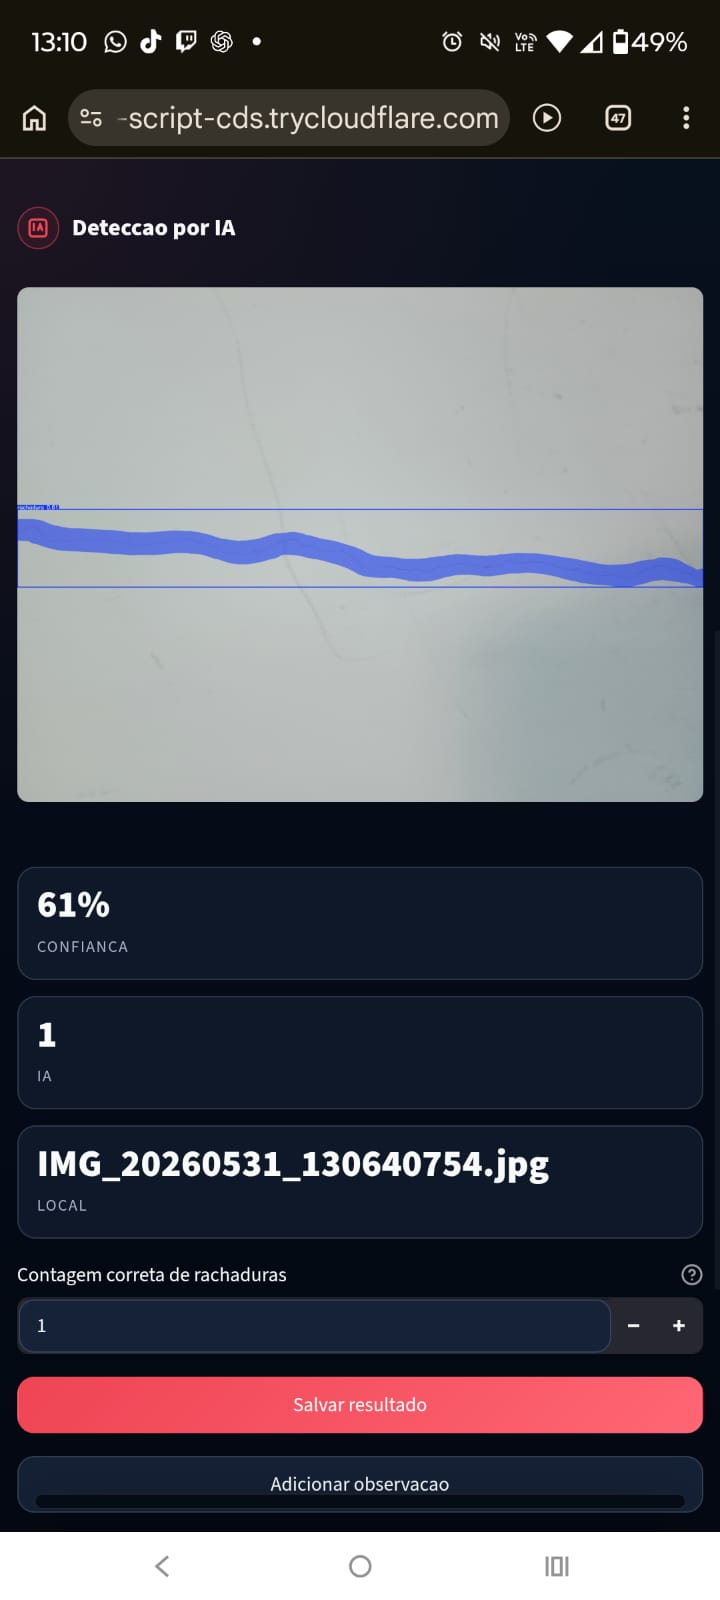
\includegraphics[width=\linewidth]{resut-1.jpeg}\caption{result-1}
  \end{subfigure}\hfill
  \begin{subfigure}{0.32\linewidth}\centering
    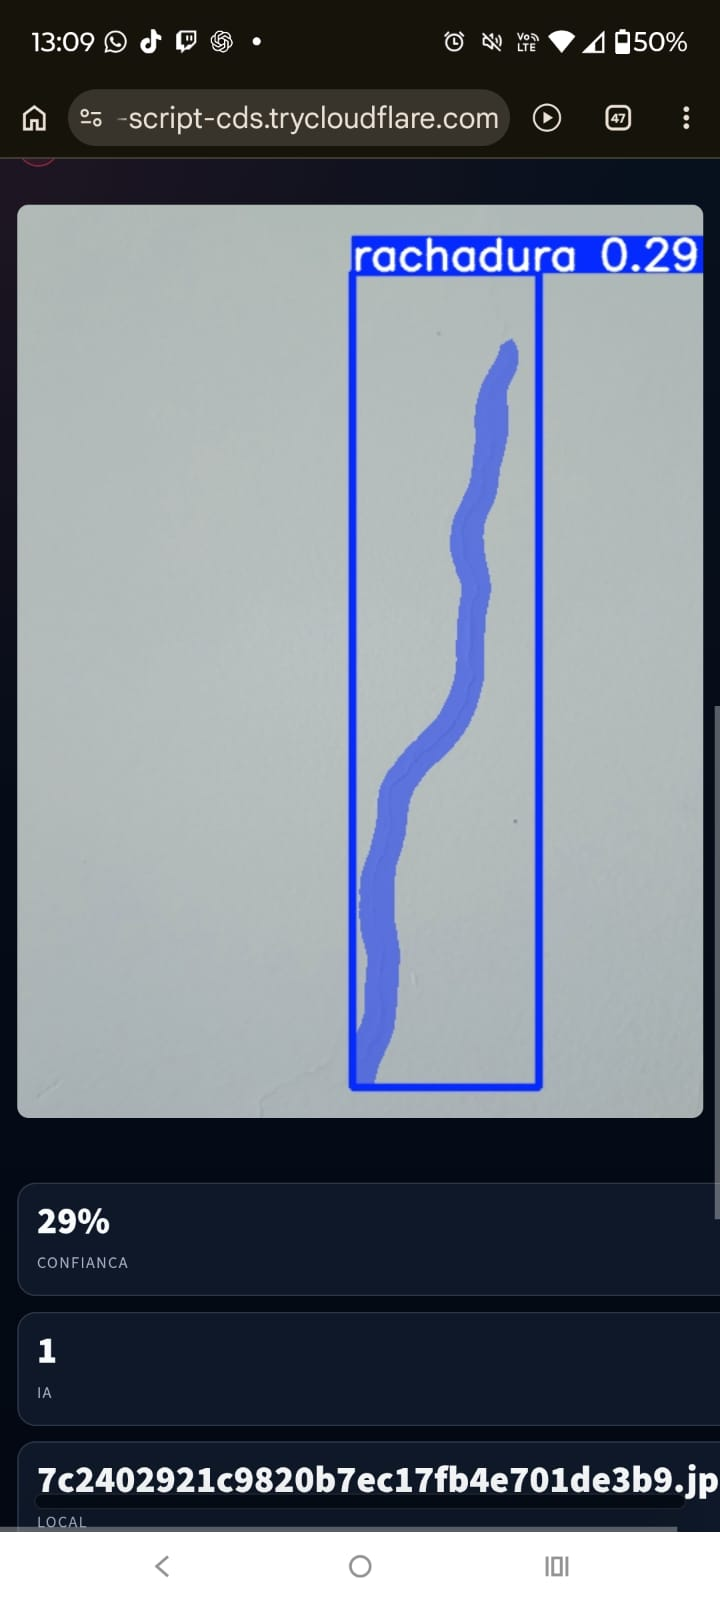
\includegraphics[width=\linewidth]{result-2.jpeg}\caption{result-2}
  \end{subfigure}\hfill
  \begin{subfigure}{0.32\linewidth}\centering
    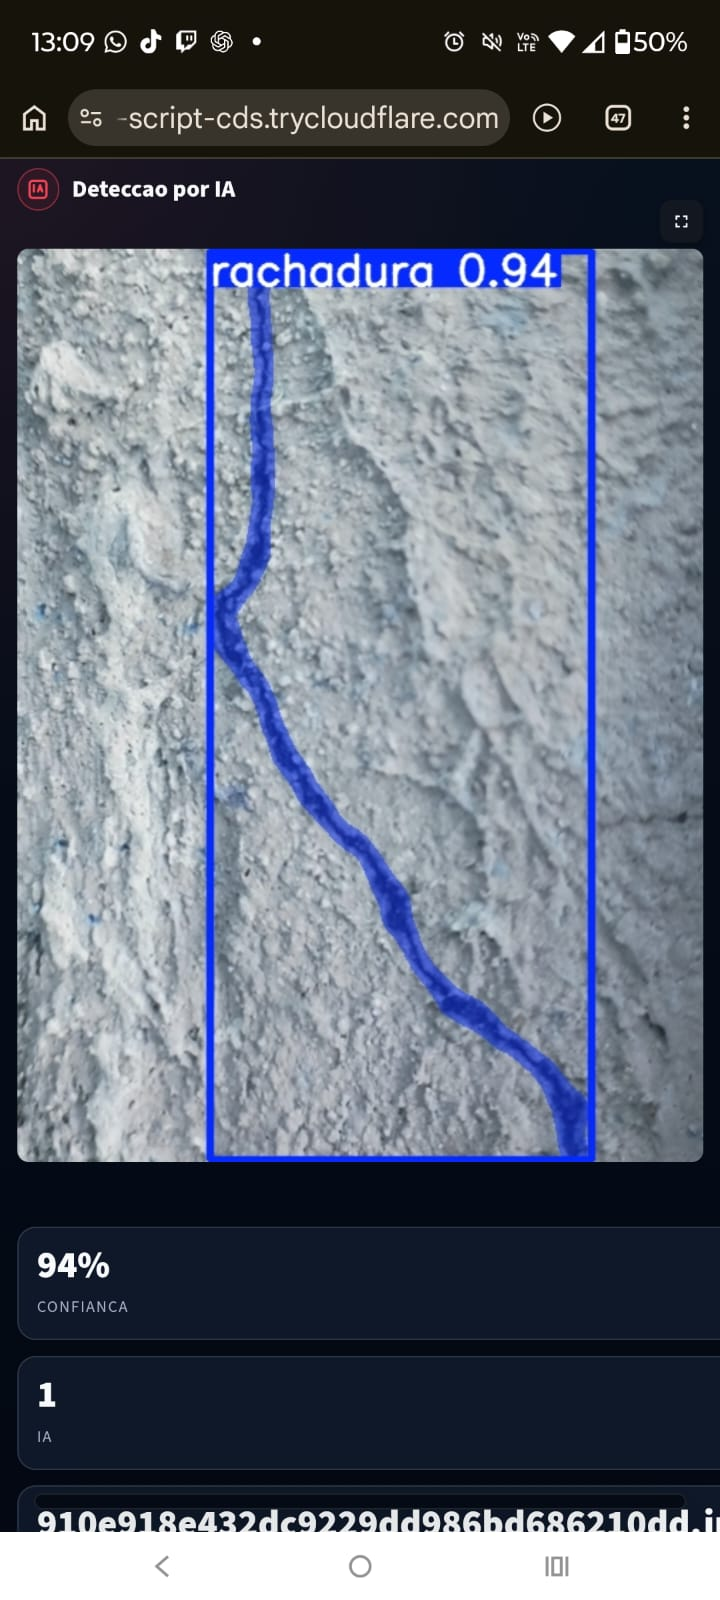
\includegraphics[width=\linewidth]{result-3.jpeg}\caption{result-3}
  \end{subfigure}
  \caption{Resultados da aplicação em imagens novas — detecção e segmentação das rachaduras.}
\end{figure}

\fig{app_test_output.jpg}{0.85}{Saída completa de teste do aplicativo (imagem original $\times$
detecção da IA com máscara e confiança).}

% ============================================================================
\section{Entrega da solução}
% ============================================================================
A entrega é composta por \textbf{três artefatos} complementares.

\begin{table}[H]\centering\small
\renewcommand{\arraystretch}{1.3}
\begin{tabular}{>{\bfseries}l >{\raggedright\arraybackslash}p{9.5cm}}
\toprule
Artefato & Descrição \\
\midrule
Aplicação web & \texttt{streamlit run app/app.py} — inspeção, histórico e dashboard. \\
Relatório técnico & Este documento (\texttt{relatorio\_tecnico\_v2.tex} / PDF). \\
Guia de implementação & PDF à parte com o planejamento de UX/UI e roteiro de implementação. \\
\bottomrule
\end{tabular}
\caption{Composição da entrega.}
\end{table}

\subsection{Guia rápido para o usuário (tela1 a tela4)}
Passo a passo para o colaborador em campo, ilustrado pelas telas do aplicativo:

\begin{enumerate}[leftmargin=1.6em]
  \item \textbf{Identifique-se} — informe nome e cargo (Tela 1).
  \item \textbf{Envie a foto} — faça upload ou use a câmera apontando para a parede (Tela 2).
  \item \textbf{Leia o resultado} — a IA marca as rachaduras com máscara e mostra confiança e
        contagem; salve a inspeção (Tela 3).
  \item \textbf{Acompanhe} — consulte o histórico/diário de obra e o dashboard por dia;
        exporte CSV se necessário (Tela 4).
\end{enumerate}

\begin{figure}[H]\centering
  \begin{subfigure}{0.48\linewidth}\centering
    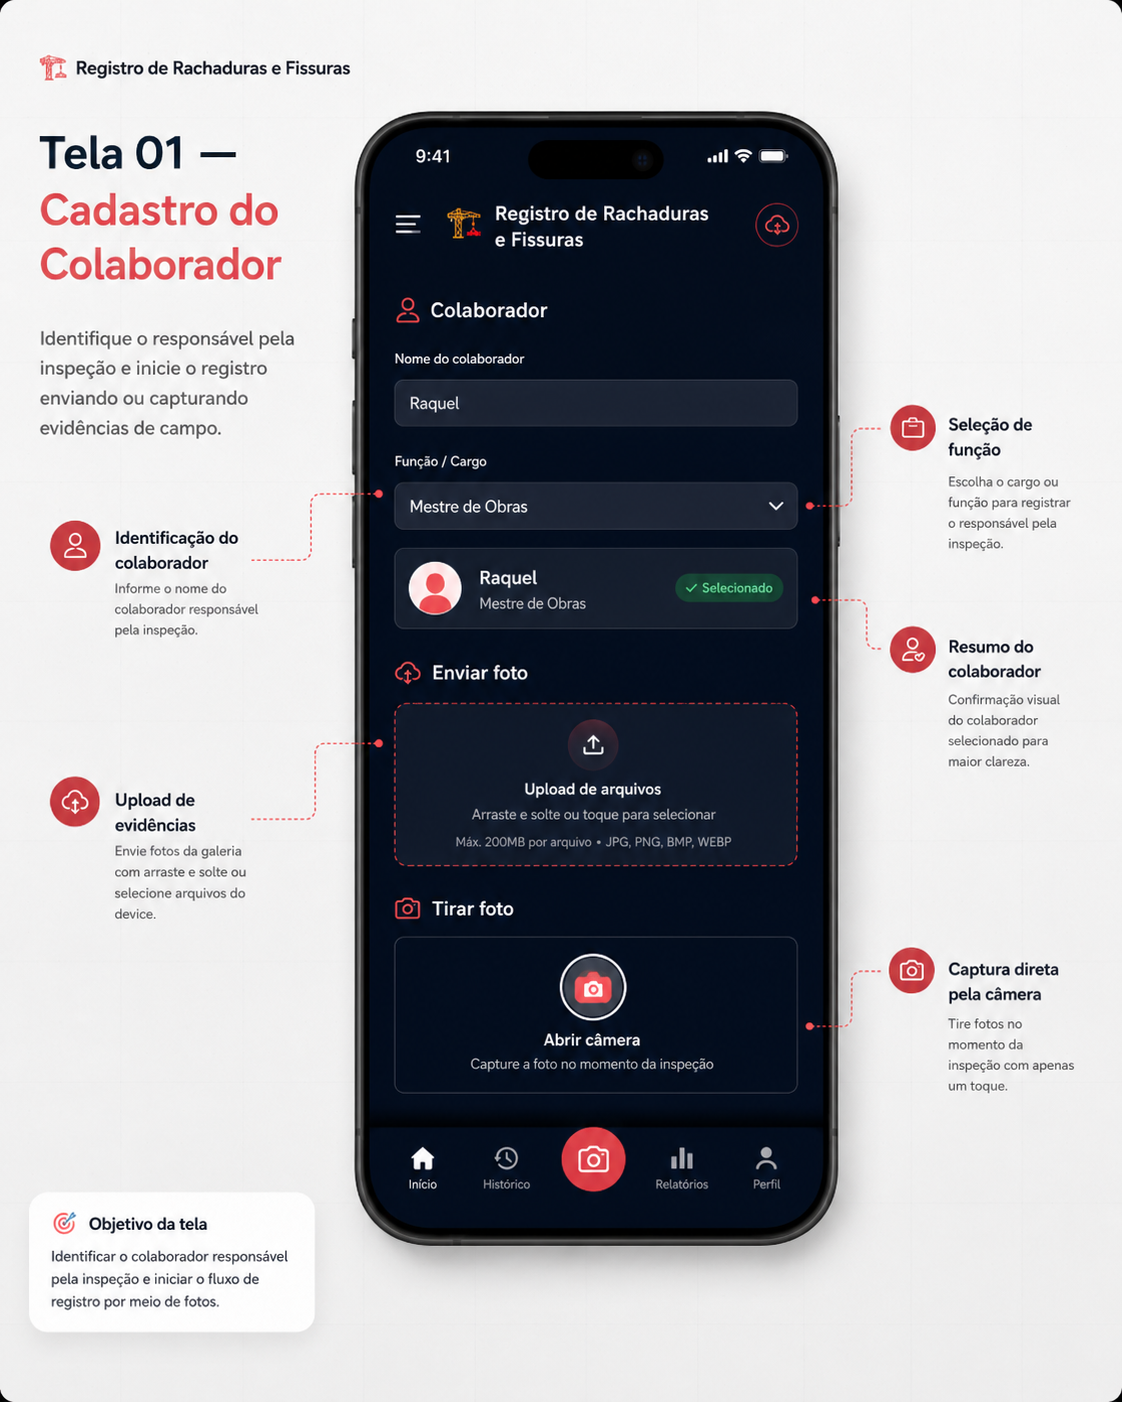
\includegraphics[width=\linewidth]{tela1.png}\caption{Passo 1 — identificação}
  \end{subfigure}\hfill
  \begin{subfigure}{0.48\linewidth}\centering
    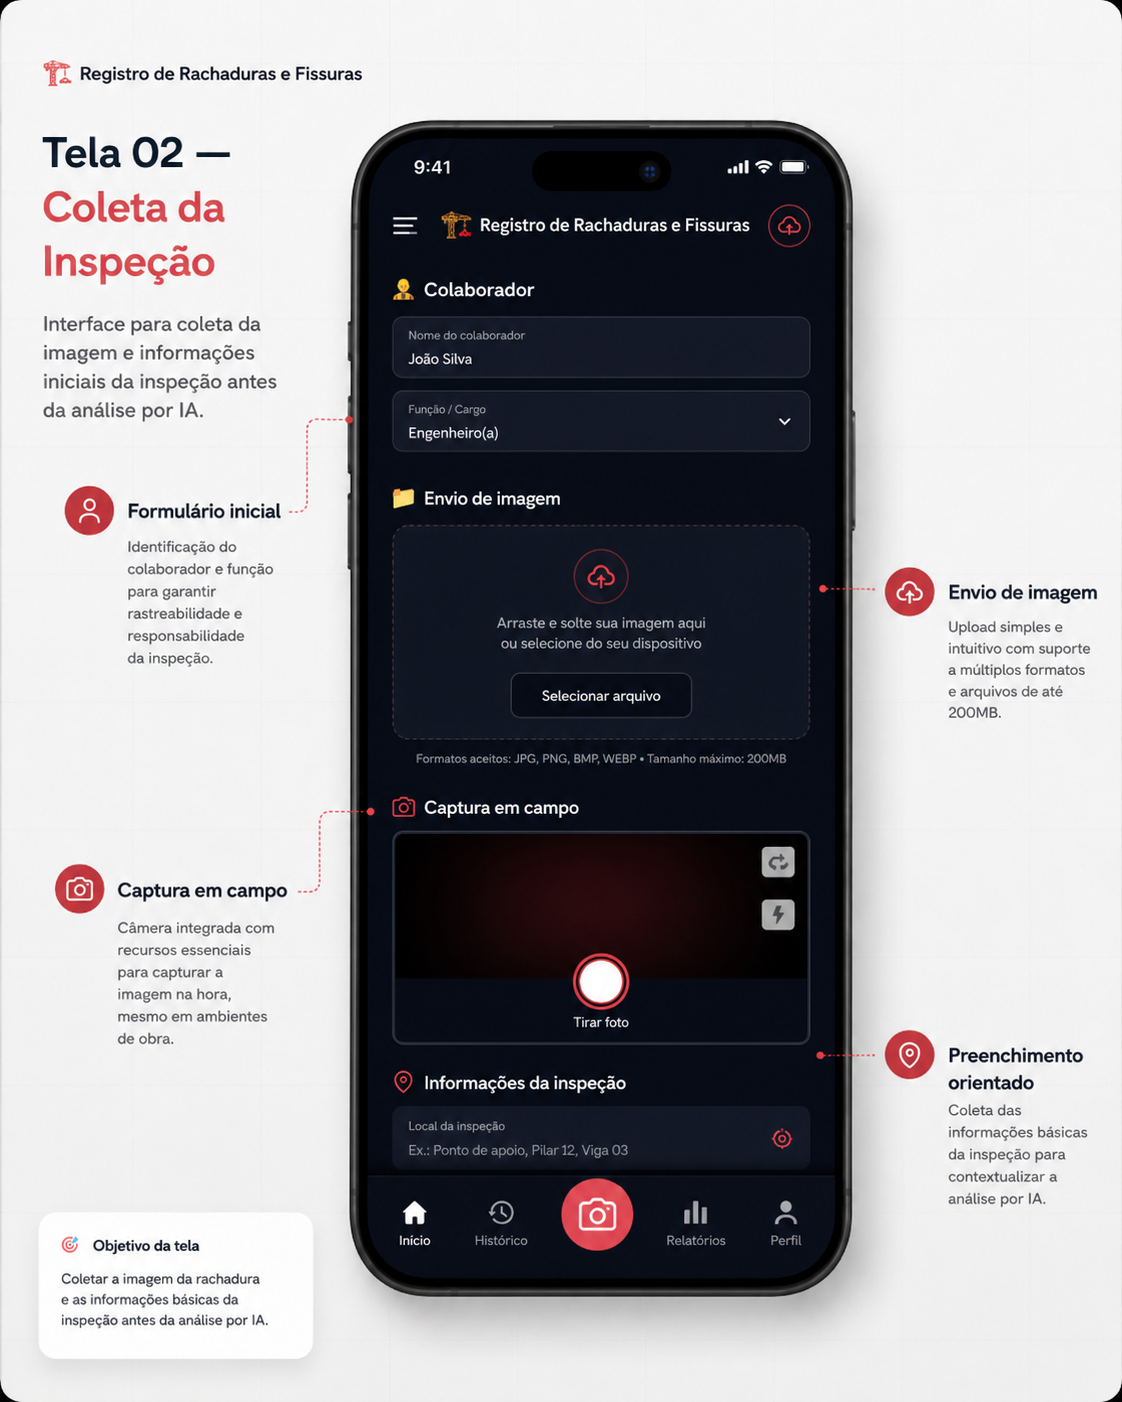
\includegraphics[width=\linewidth]{tela2.png}\caption{Passo 2 — envio da imagem}
  \end{subfigure}
  \\[6pt]
  \begin{subfigure}{0.48\linewidth}\centering
    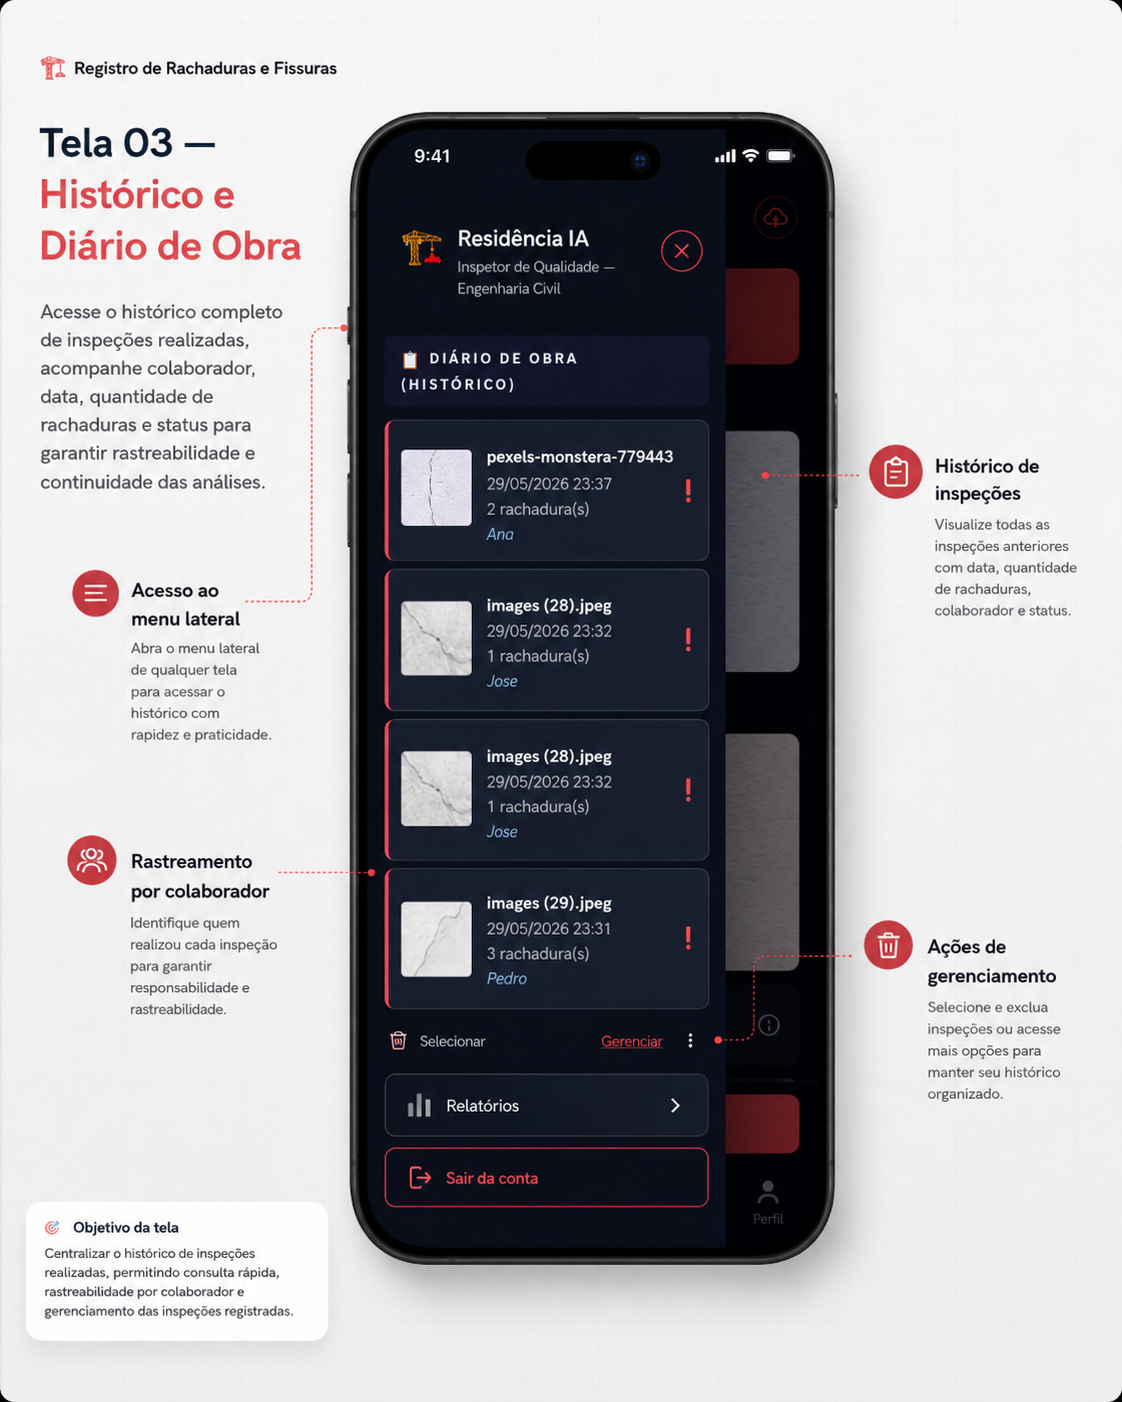
\includegraphics[width=\linewidth]{tela3.png}\caption{Passo 3 — resultado e registro}
  \end{subfigure}\hfill
  \begin{subfigure}{0.48\linewidth}\centering
    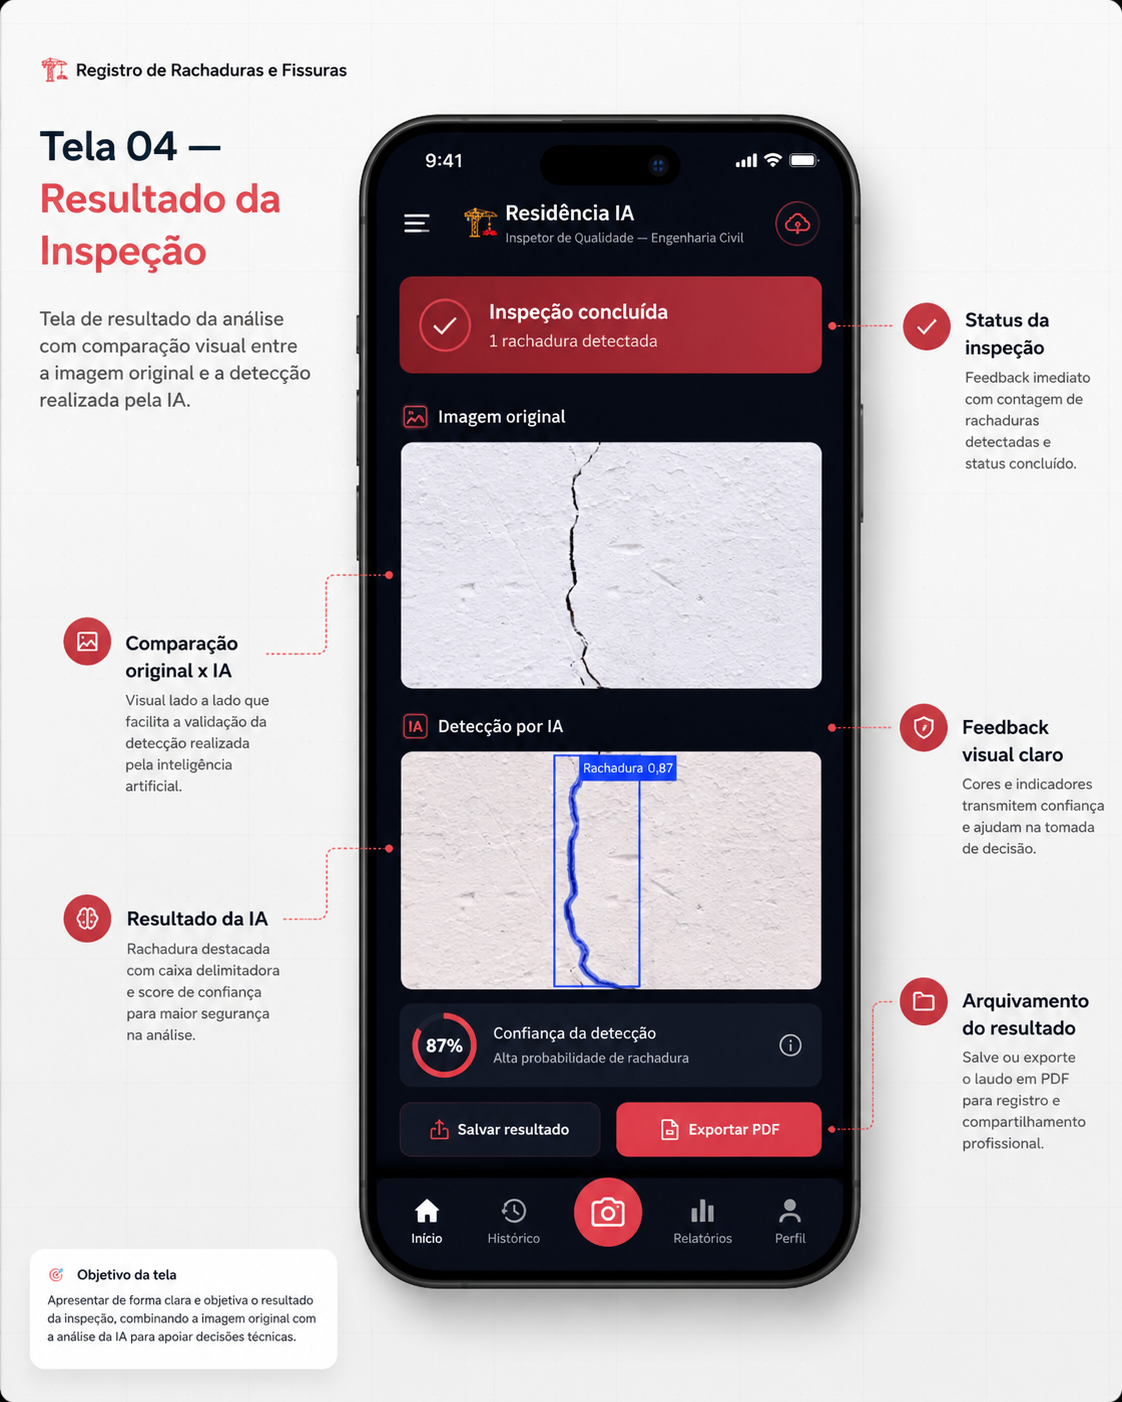
\includegraphics[width=\linewidth]{tela4.png}\caption{Passo 4 — histórico e dashboard}
  \end{subfigure}
  \caption{Guia visual do usuário — fluxo completo de uso (tela1 a tela4).}
\end{figure}

\fig{guia-do-usuario.png}{0.9}{Guia do usuário consolidado.}

\subsection{Guia de planejamento de implementação (PDF à parte)}
O detalhamento do \textbf{planejamento de implementação e do projeto de UX/UI} é entregue como
um \textbf{documento PDF separado}:
\begin{infobox}
\textbf{Arquivo:} \texttt{guia\_ux\_ui\_registro\_rachaduras\_fissuras.pdf}\\
Conteúdo: jornada do usuário, decisões de design, protótipos (tela1--tela4), arquitetura da
aplicação e roteiro de evolução (incluindo a integração futura com SAM\,3 caso haja recurso).
\end{infobox}

% ============================================================================
\section{Conclusão e próximos passos}
% ============================================================================
A solução cumpre o Desafio 2: detecta e segmenta rachaduras com \textbf{mAP@0.5 = 75,8\%} e
\textbf{Precision = 86,8\%} (caixa, teste), embarcada em um aplicativo prático de inspeção com
histórico e dashboard, e com caminho de deploy \emph{edge} via ONNX/TFLite.

\paragraph{Próximos passos.}
\begin{itemize}[leftmargin=1.4em]
  \item Ampliar e diversificar o dataset (mais texturas/iluminações) para elevar o recall.
  \item Classificar severidade da fissura (largura/comprimento estimados).
  \item Em fase com mais recurso, avaliar \textbf{SAM\,3} para casos difíceis e rotulagem
        assistida, em arquitetura híbrida com o YOLO nano em campo.
\end{itemize}

\vfill
\begin{center}\small\color{graytxt}
Relatório Técnico v2 — Desafio 2 — Detecção de Trincas e Fissuras em Paredes
\end{center}

\end{document}
